\documentclass{beamer}

\usepackage{fontspec,xunicode,xltxtra}
\usepackage[english]{babel}
\usepackage{microtype}
\usepackage{default}	

\usepackage[]{hyperref}
\hypersetup{
	colorlinks=true}
\usetheme{simple}
\usepackage{graphicx}
\usepackage[utf8]{inputenc}
\usepackage[justification=centering]{caption}
\usepackage{subcaption}
\usepackage{listings}
\usepackage{pstricks}
\setmainfont{Fira Sans}
\setsansfont{Noto Sans}
\setmonofont{Fira Mono}
\captionsetup[subfigure]{labelformat=empty}
\captionsetup[figure]{labelformat=empty}
\setbeamertemplate{caption}{\raggedright\insertcaption\par}
\setbeamerfont{frametitle}{size=\LARGE}
\newfontfamily\DejaSans{DejaVu Sans}
\setbeamerfont{title}{family=\texttt,size=\huge}
\usepackage[scale=2]{ccicons}
\newfontfamily\unicodefun[Ligatures=TeX]{Symbola}
\newfontfamily\unicodefun{Droid Sans}
\title{Rethinking the DAW paradigm}
\subtitle{With i-score \& the LibAudioStream}
\date{}
\author{Jean-Michaël Celerier~\\ Myriam Desainte-Catherine~\\ Jean-Michel Couturier}
\institute{LaBRI, Blue Yeti}
\usepackage{tikz}

\newsavebox{\codebox}% For storing listings
\begin{document}
    
\maketitle
\begin{frame}
	\tableofcontents
\end{frame}
\section{Introduction}

\begin{frame}
    \frametitle{DAWs}    
    \Large
    \begin{figure}
        \centering
        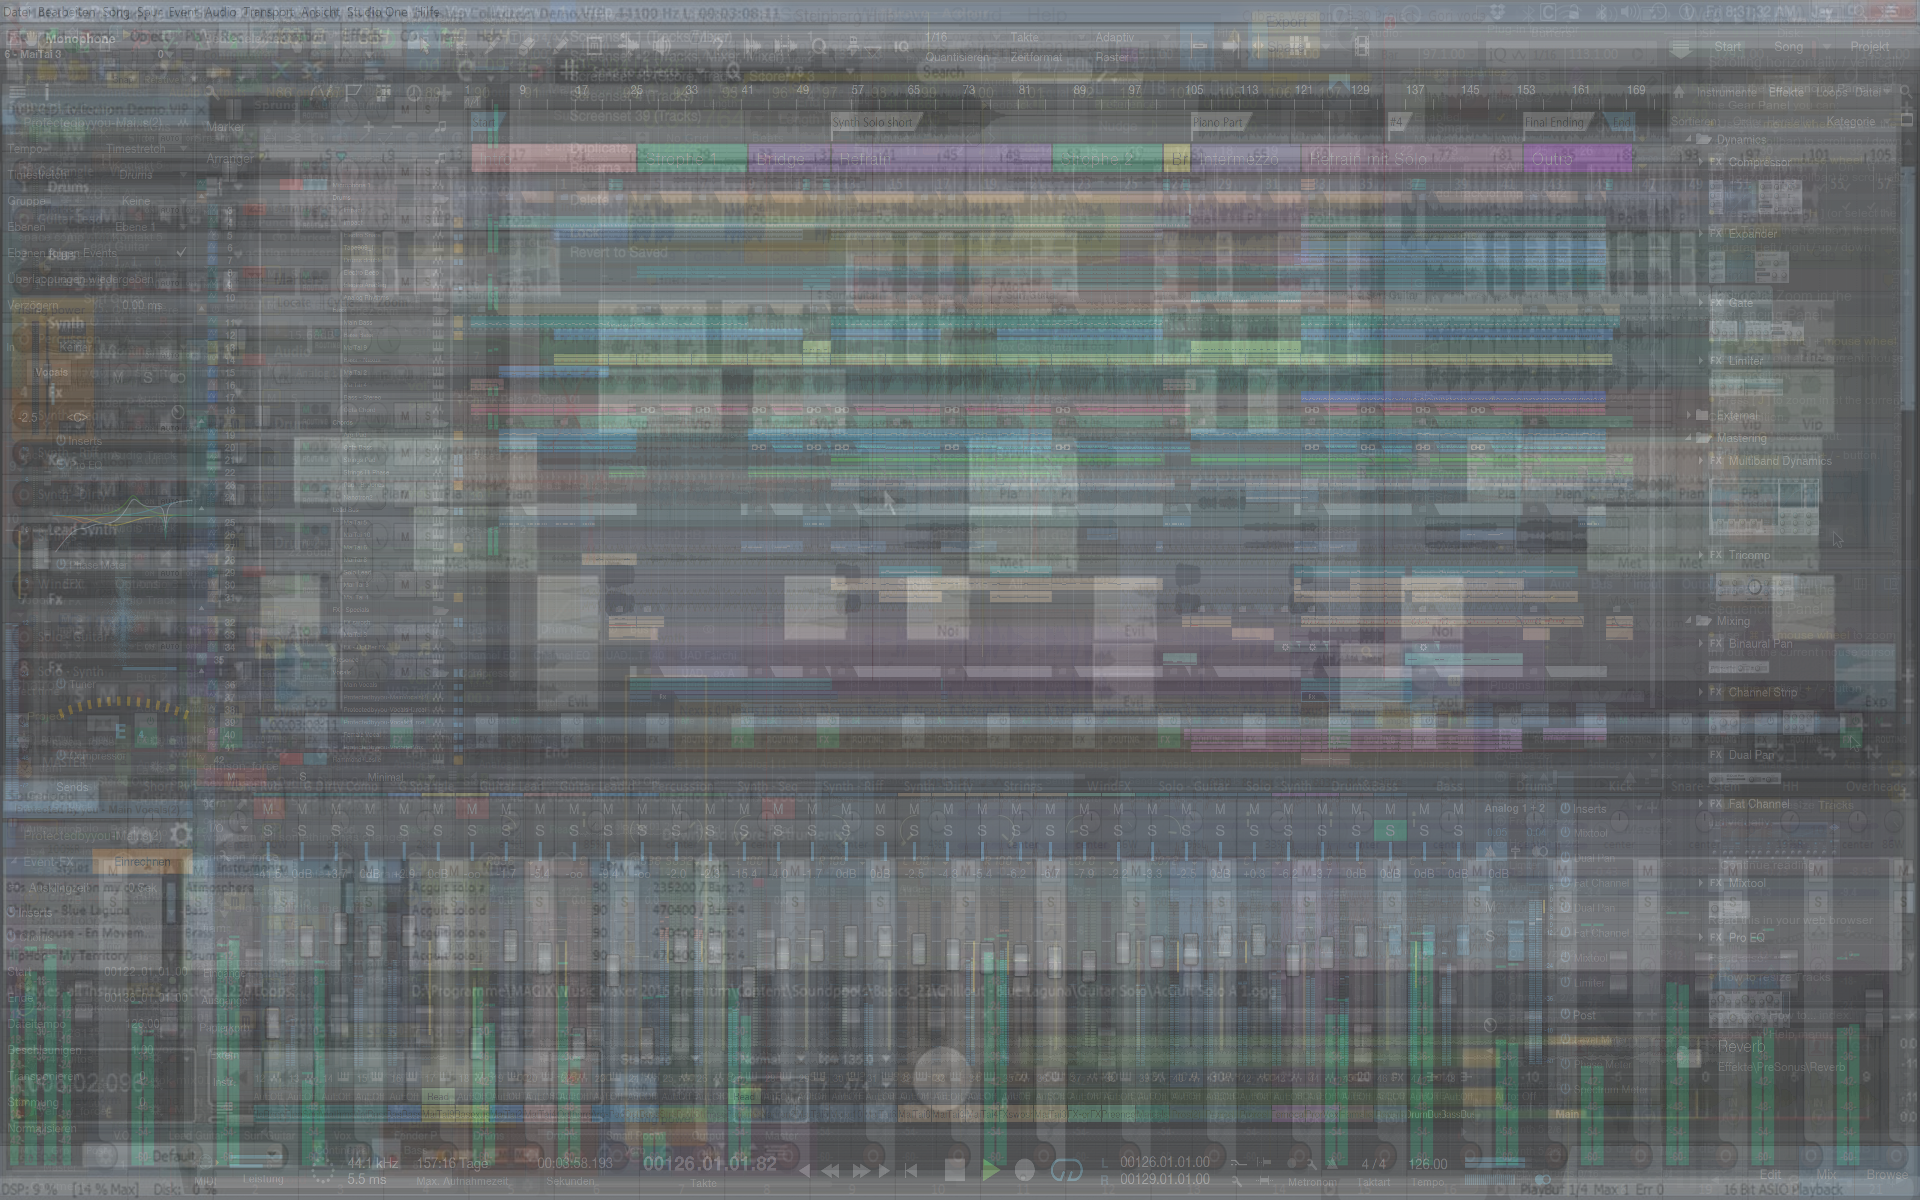
\includegraphics[width=0.9\textwidth]{images/daws/together-flattened.png}
        \caption{"Mixing"}
    \end{figure}
\end{frame}

\begin{frame}
    \frametitle{DAWs}    
    \Large
    \begin{figure}
        \centering
        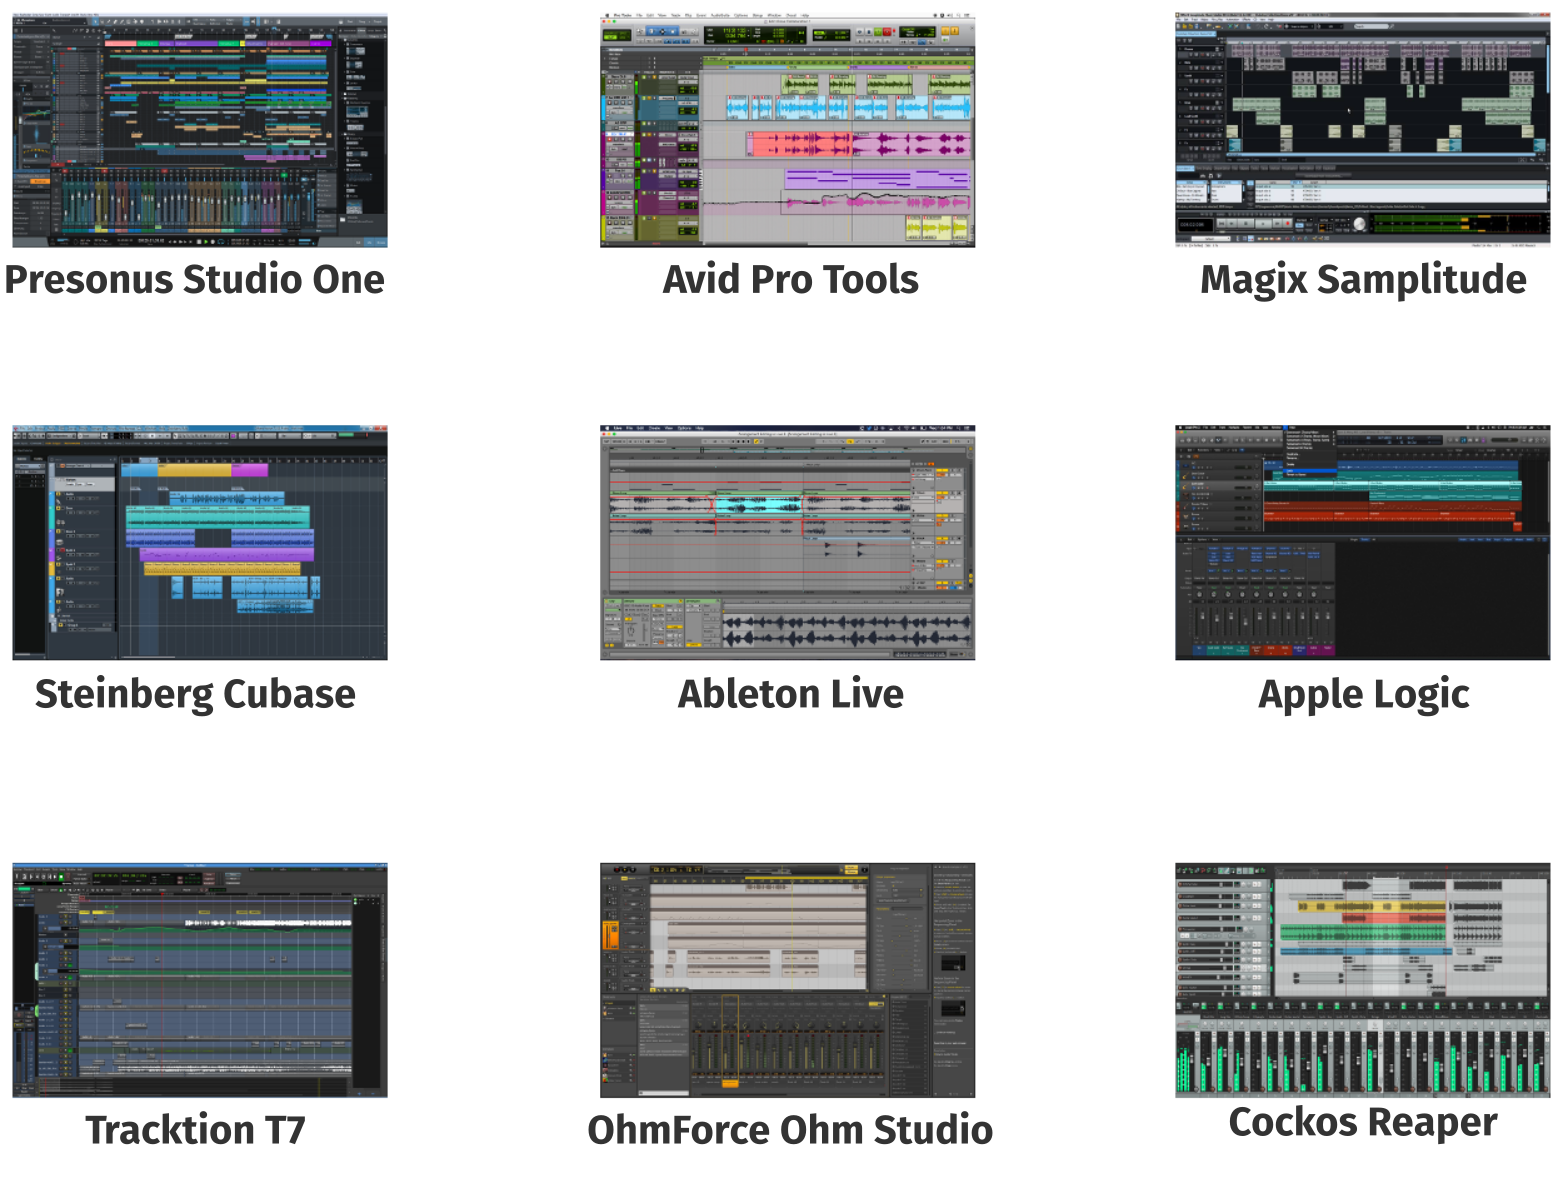
\includegraphics[width=0.7\textwidth]{images/daws/together-text.png}
        \caption{Pre-mix}
    \end{figure}
\end{frame}

\begin{frame}
	\frametitle{Music software UIs}    
	\Large
	\begin{itemize}
        \item<1-> Skeuomorphic (Most DAWs).
		\item<2-> Dataflows (\textbf{PureData}, \textbf{Max}, \textbf{OpenMusic}, \dots)
		\item<3-> Text (\textbf{Csound}, \textbf{ChucK}, \textbf{SuperCol}, \textbf{Nyquist}, \dots)
		\item<4-> Sometimes multiple possibilities~\\ (\textbf{Kyma}, \textbf{Antescofo}, \dots)
        \item<5-> Many others !
        \item<6-> Most are open for extensibility.
	\end{itemize}
\end{frame}

\begin{frame}
	\Huge
    \centering
    \textbf{What if...}
\end{frame}

\begin{frame}[plain]
    \begin{tikzpicture}[remember picture,overlay]
    \node[at=(current page.center)] {
        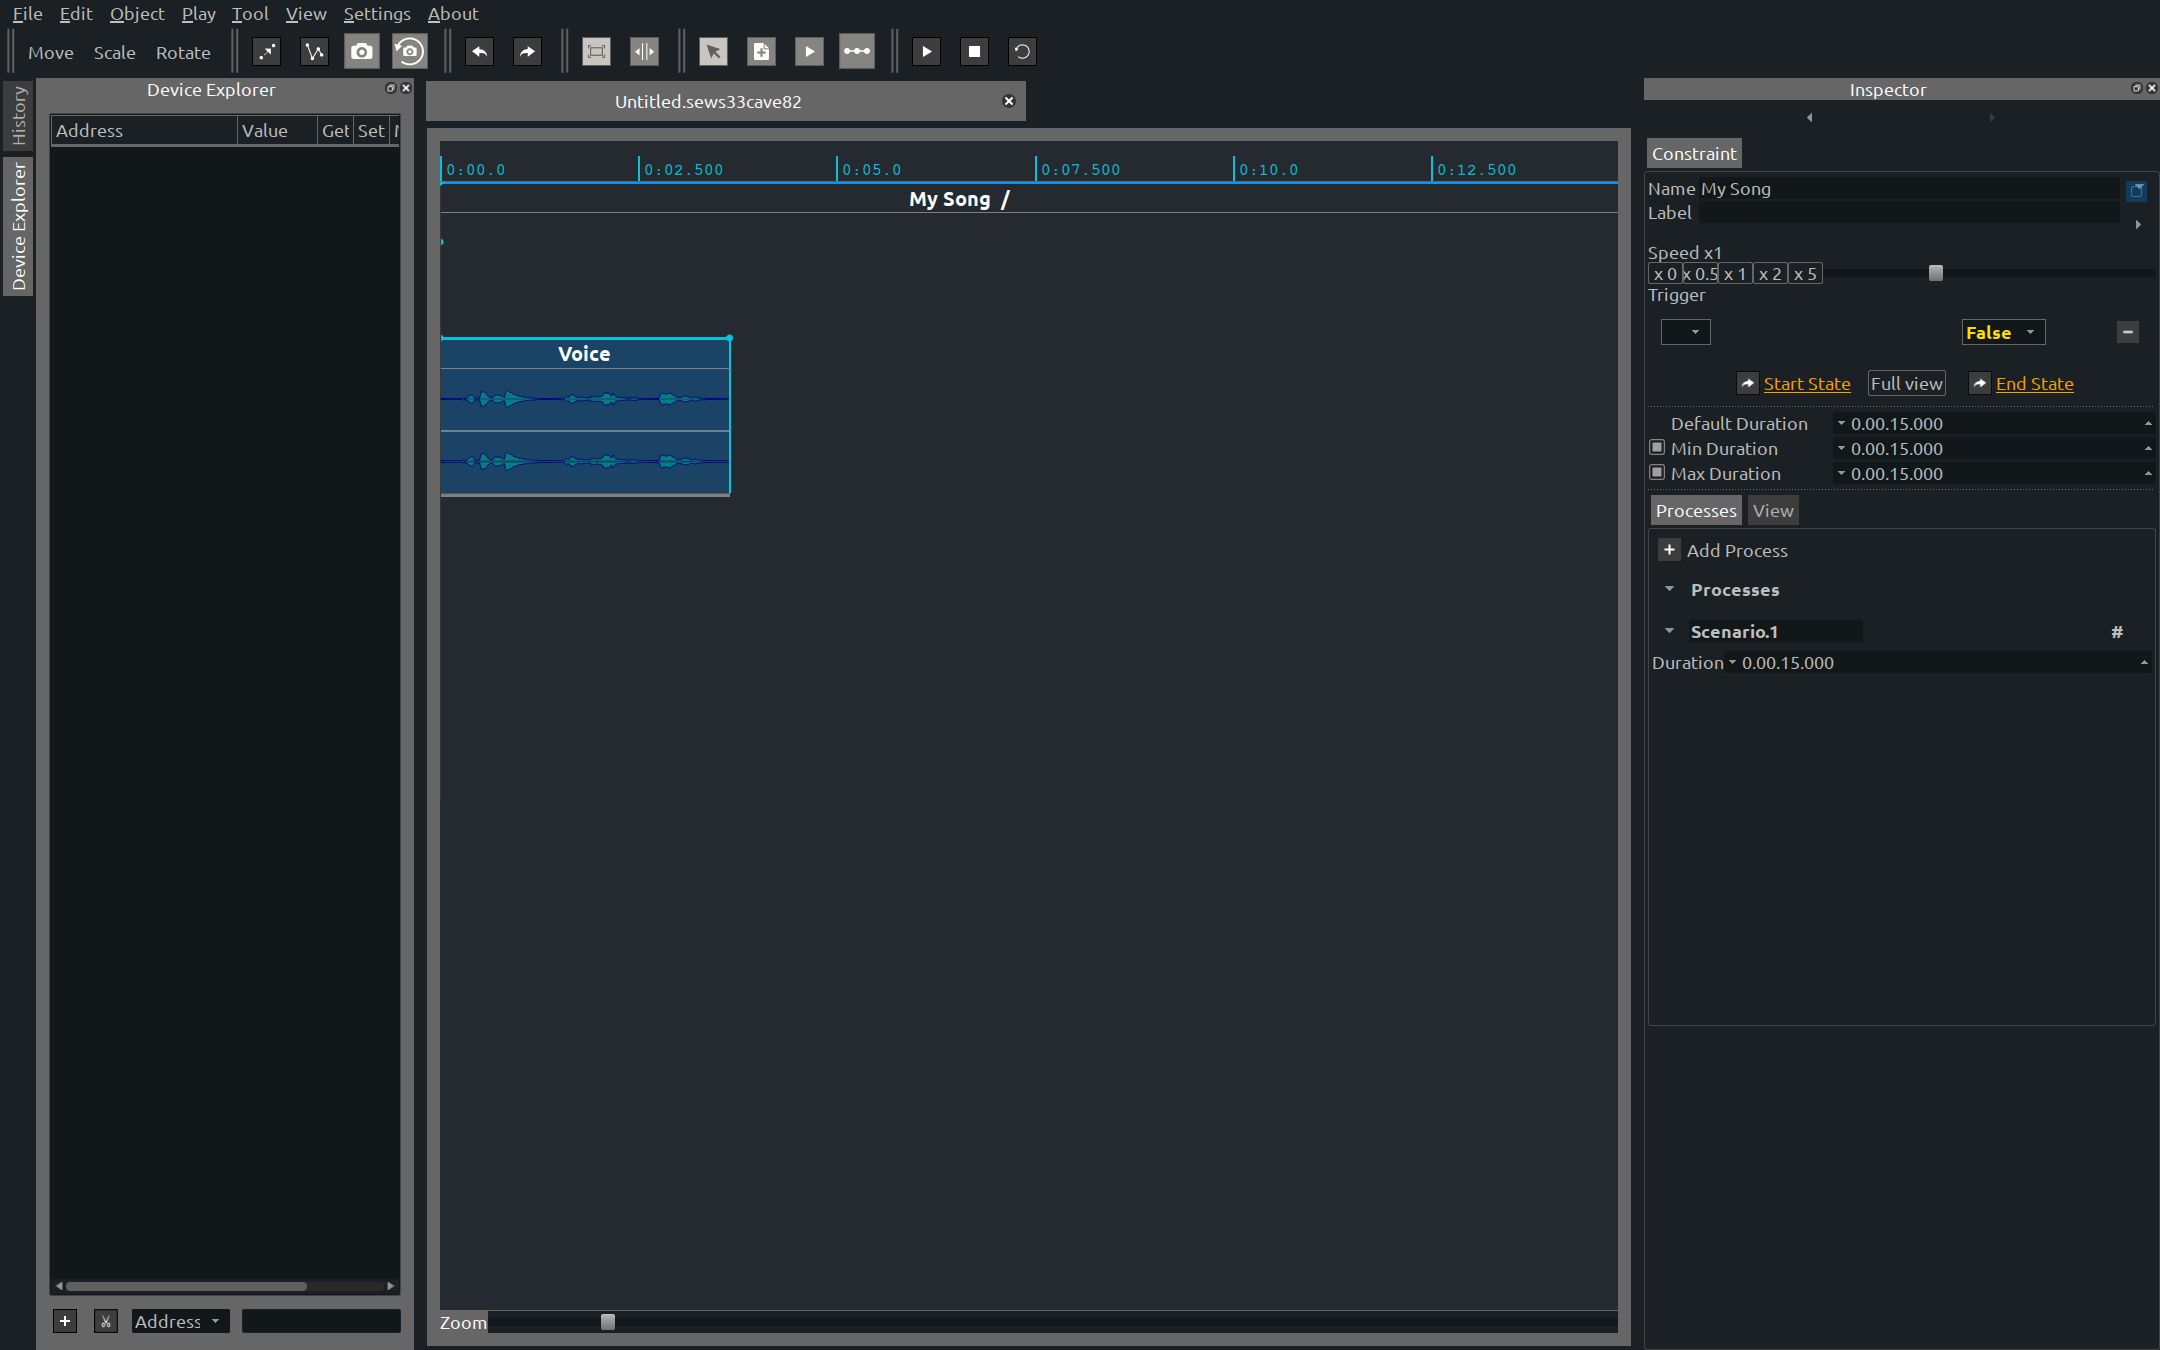
\includegraphics[width=\paperwidth]{images/screens/1.png}
    };
    \end{tikzpicture}
\end{frame}

\begin{frame}[plain]
    \begin{tikzpicture}[remember picture,overlay]
    \node[at=(current page.center)] {
        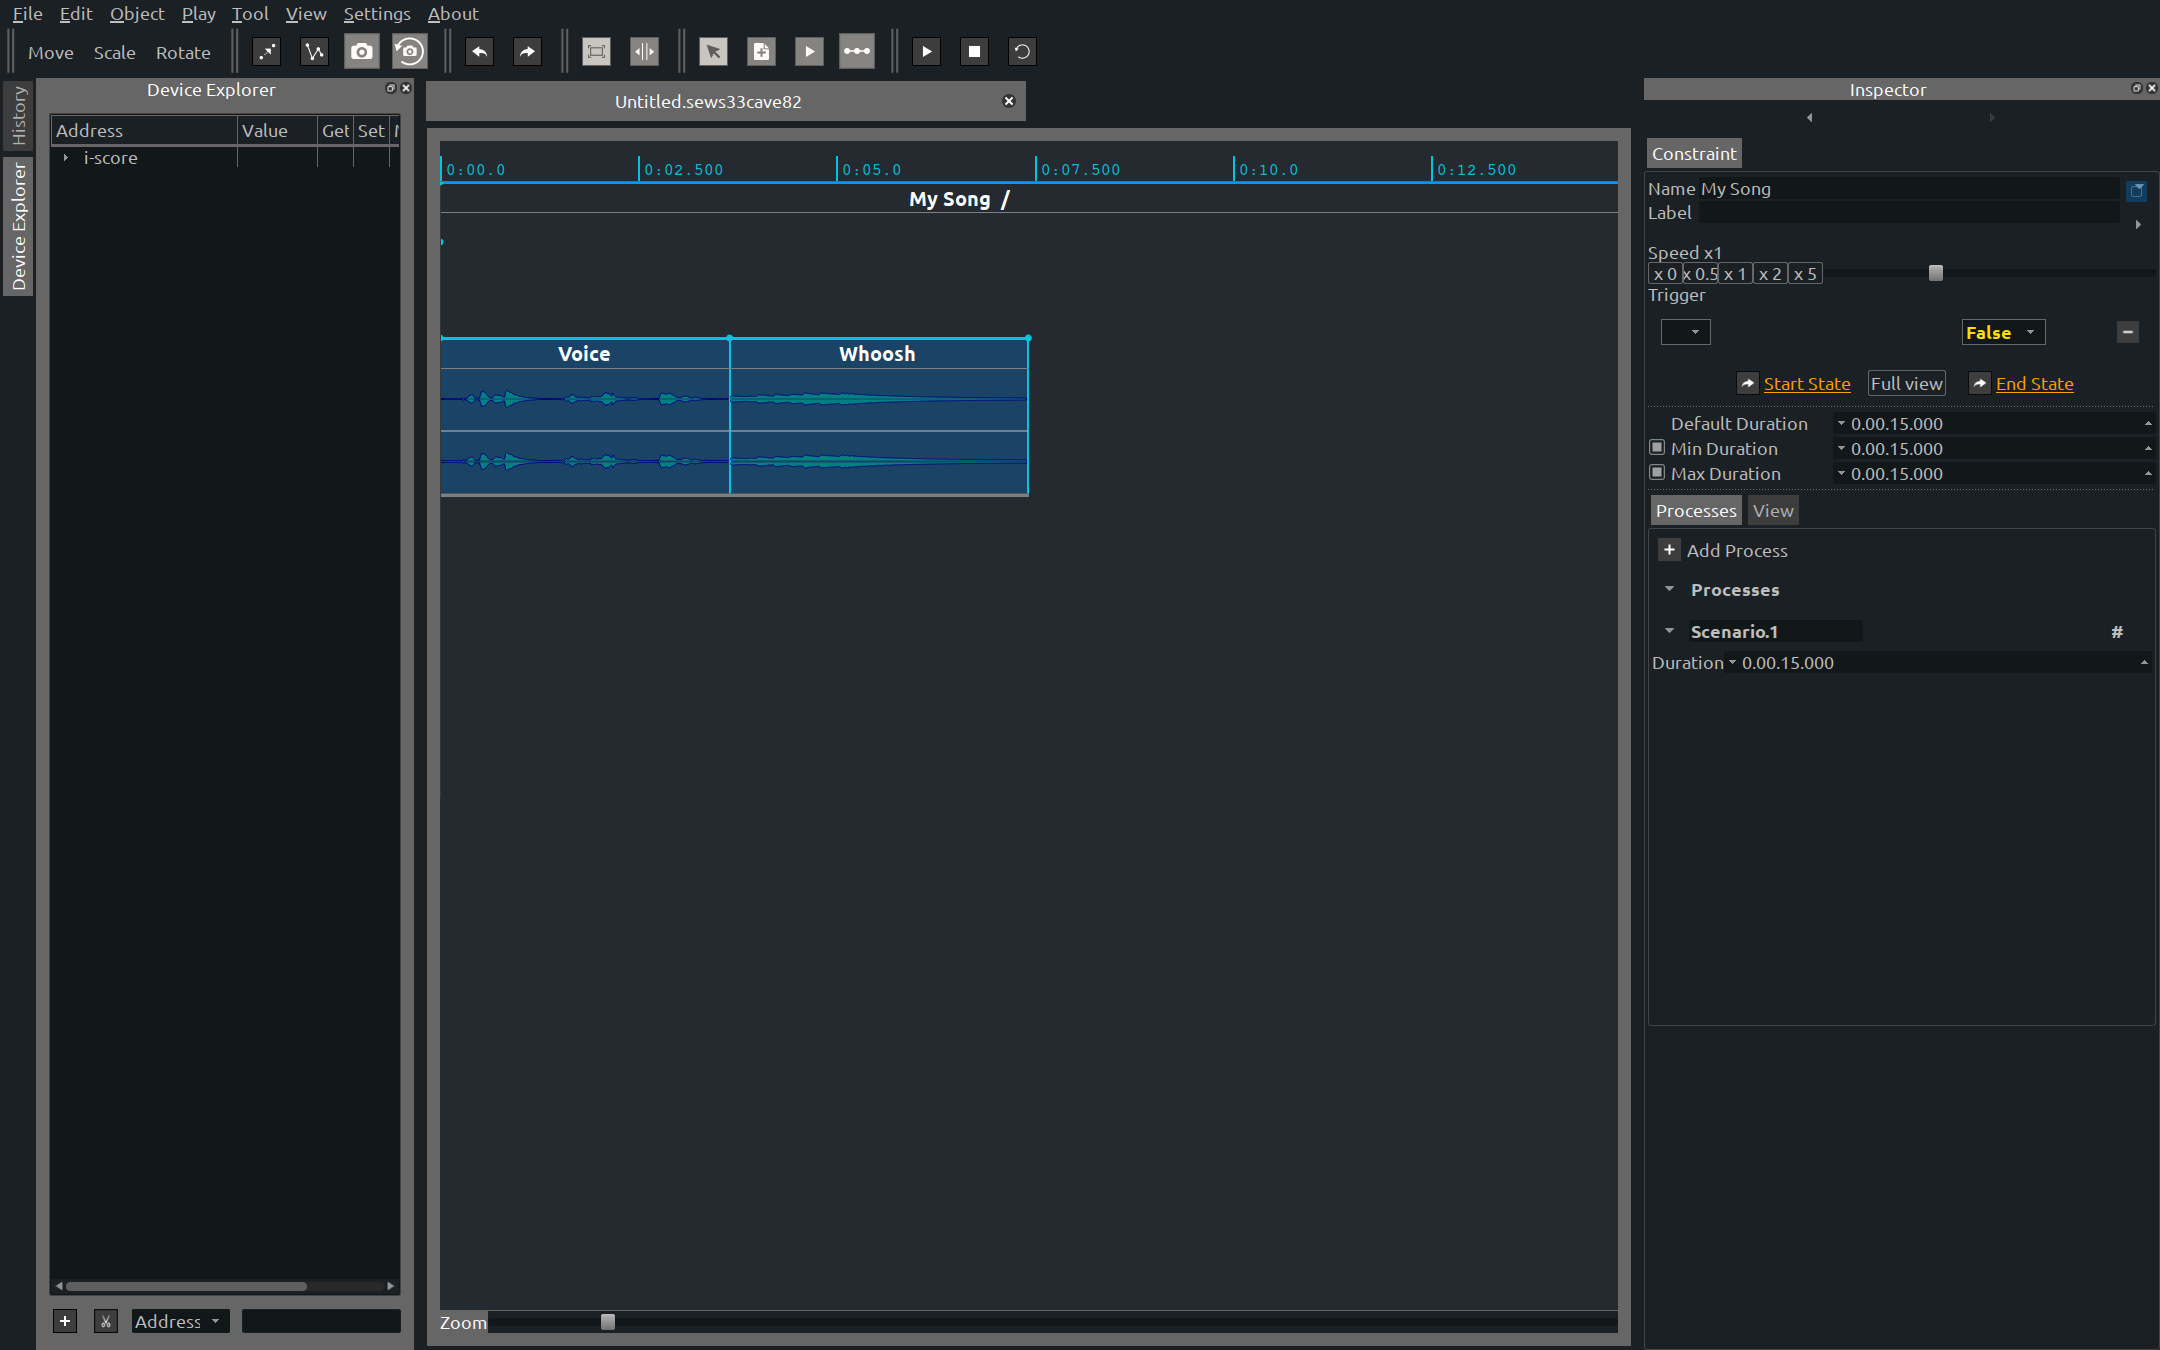
\includegraphics[width=\paperwidth]{images/screens/2.png}
    };
    \end{tikzpicture}
\end{frame}

\begin{frame}[plain]
    \begin{tikzpicture}[remember picture,overlay]
    \node[at=(current page.center)] {
        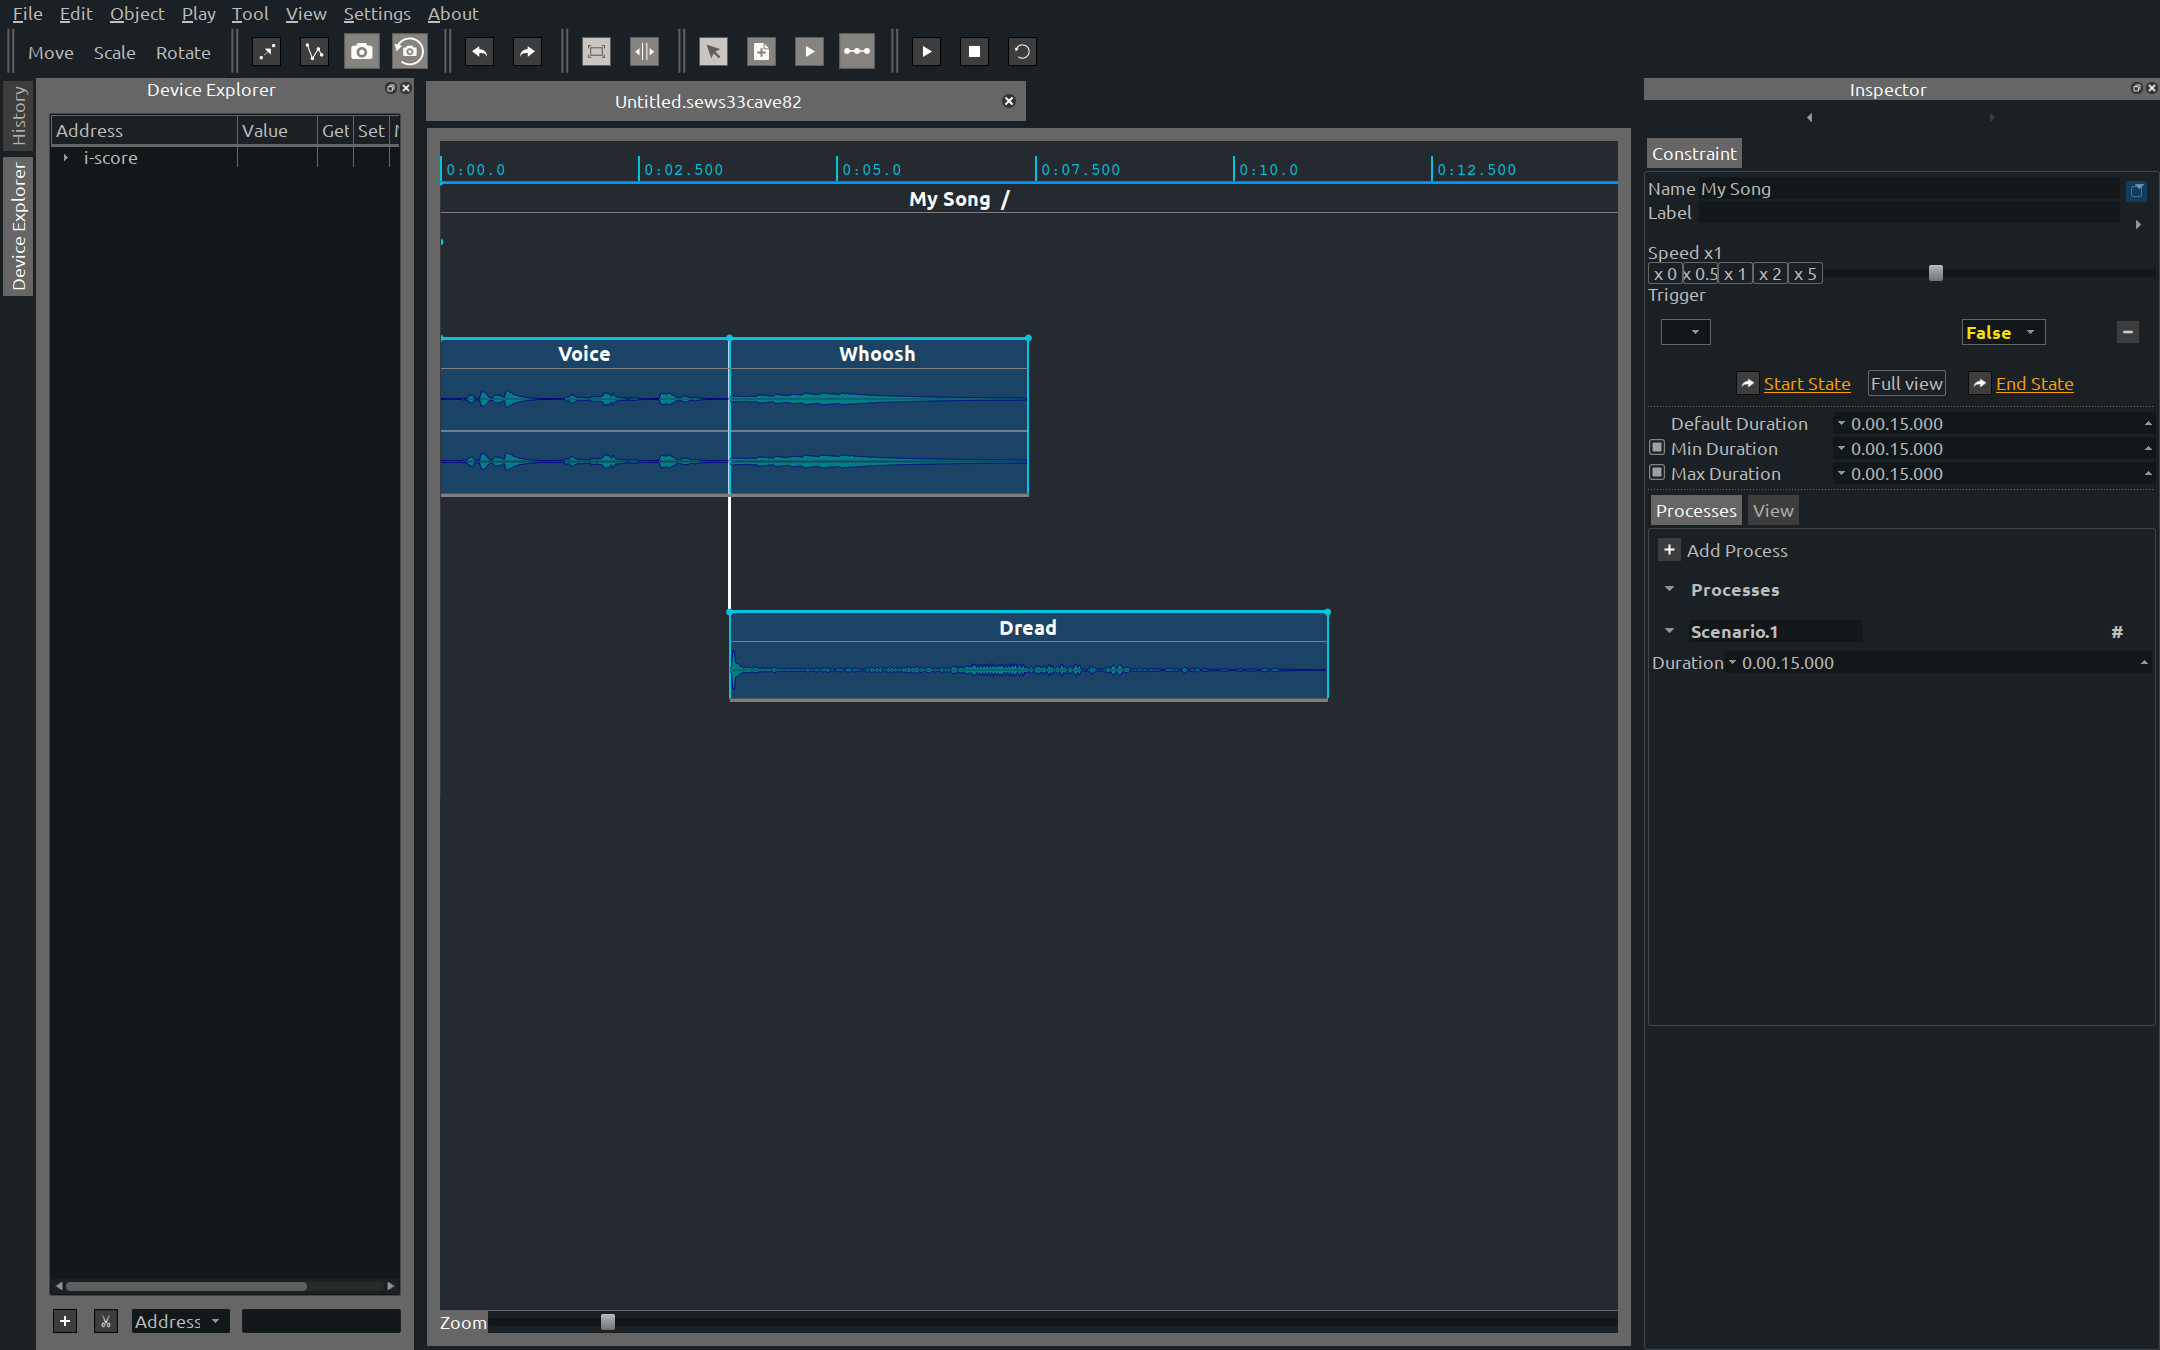
\includegraphics[width=\paperwidth]{images/screens/3.png}
    };
    \end{tikzpicture}
\end{frame}
\begin{frame}[plain]
    \begin{tikzpicture}[remember picture,overlay]
    \node[at=(current page.center)] {
        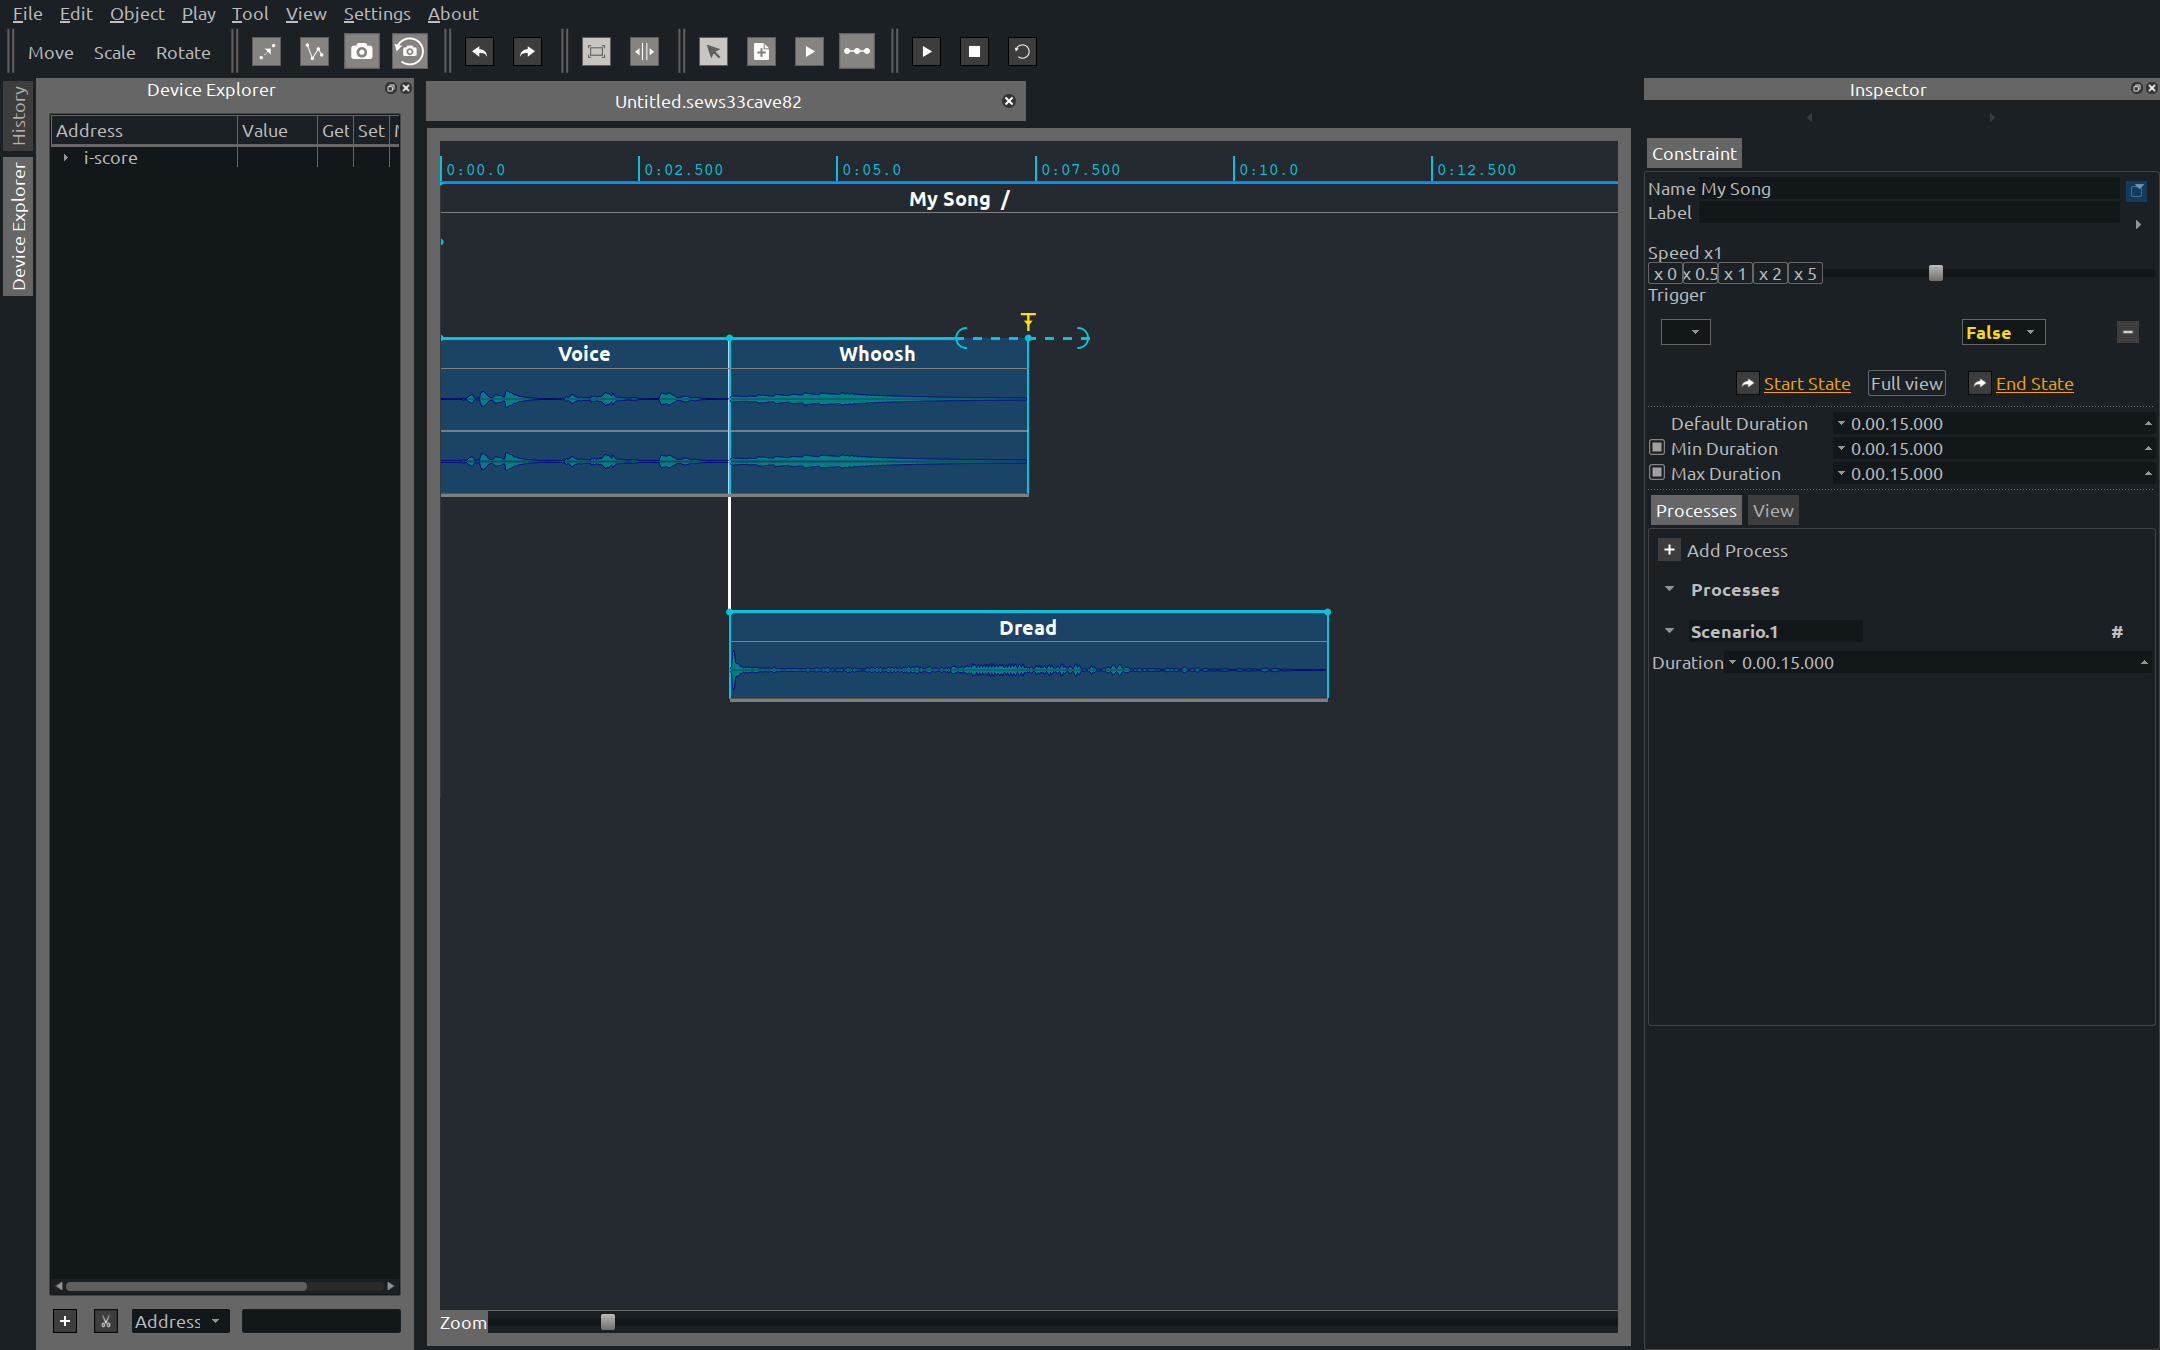
\includegraphics[width=\paperwidth]{images/screens/4.png}
    };
    \end{tikzpicture}
\end{frame}
\begin{frame}[plain]
    \begin{tikzpicture}[remember picture,overlay]
    \node[at=(current page.center)] {
        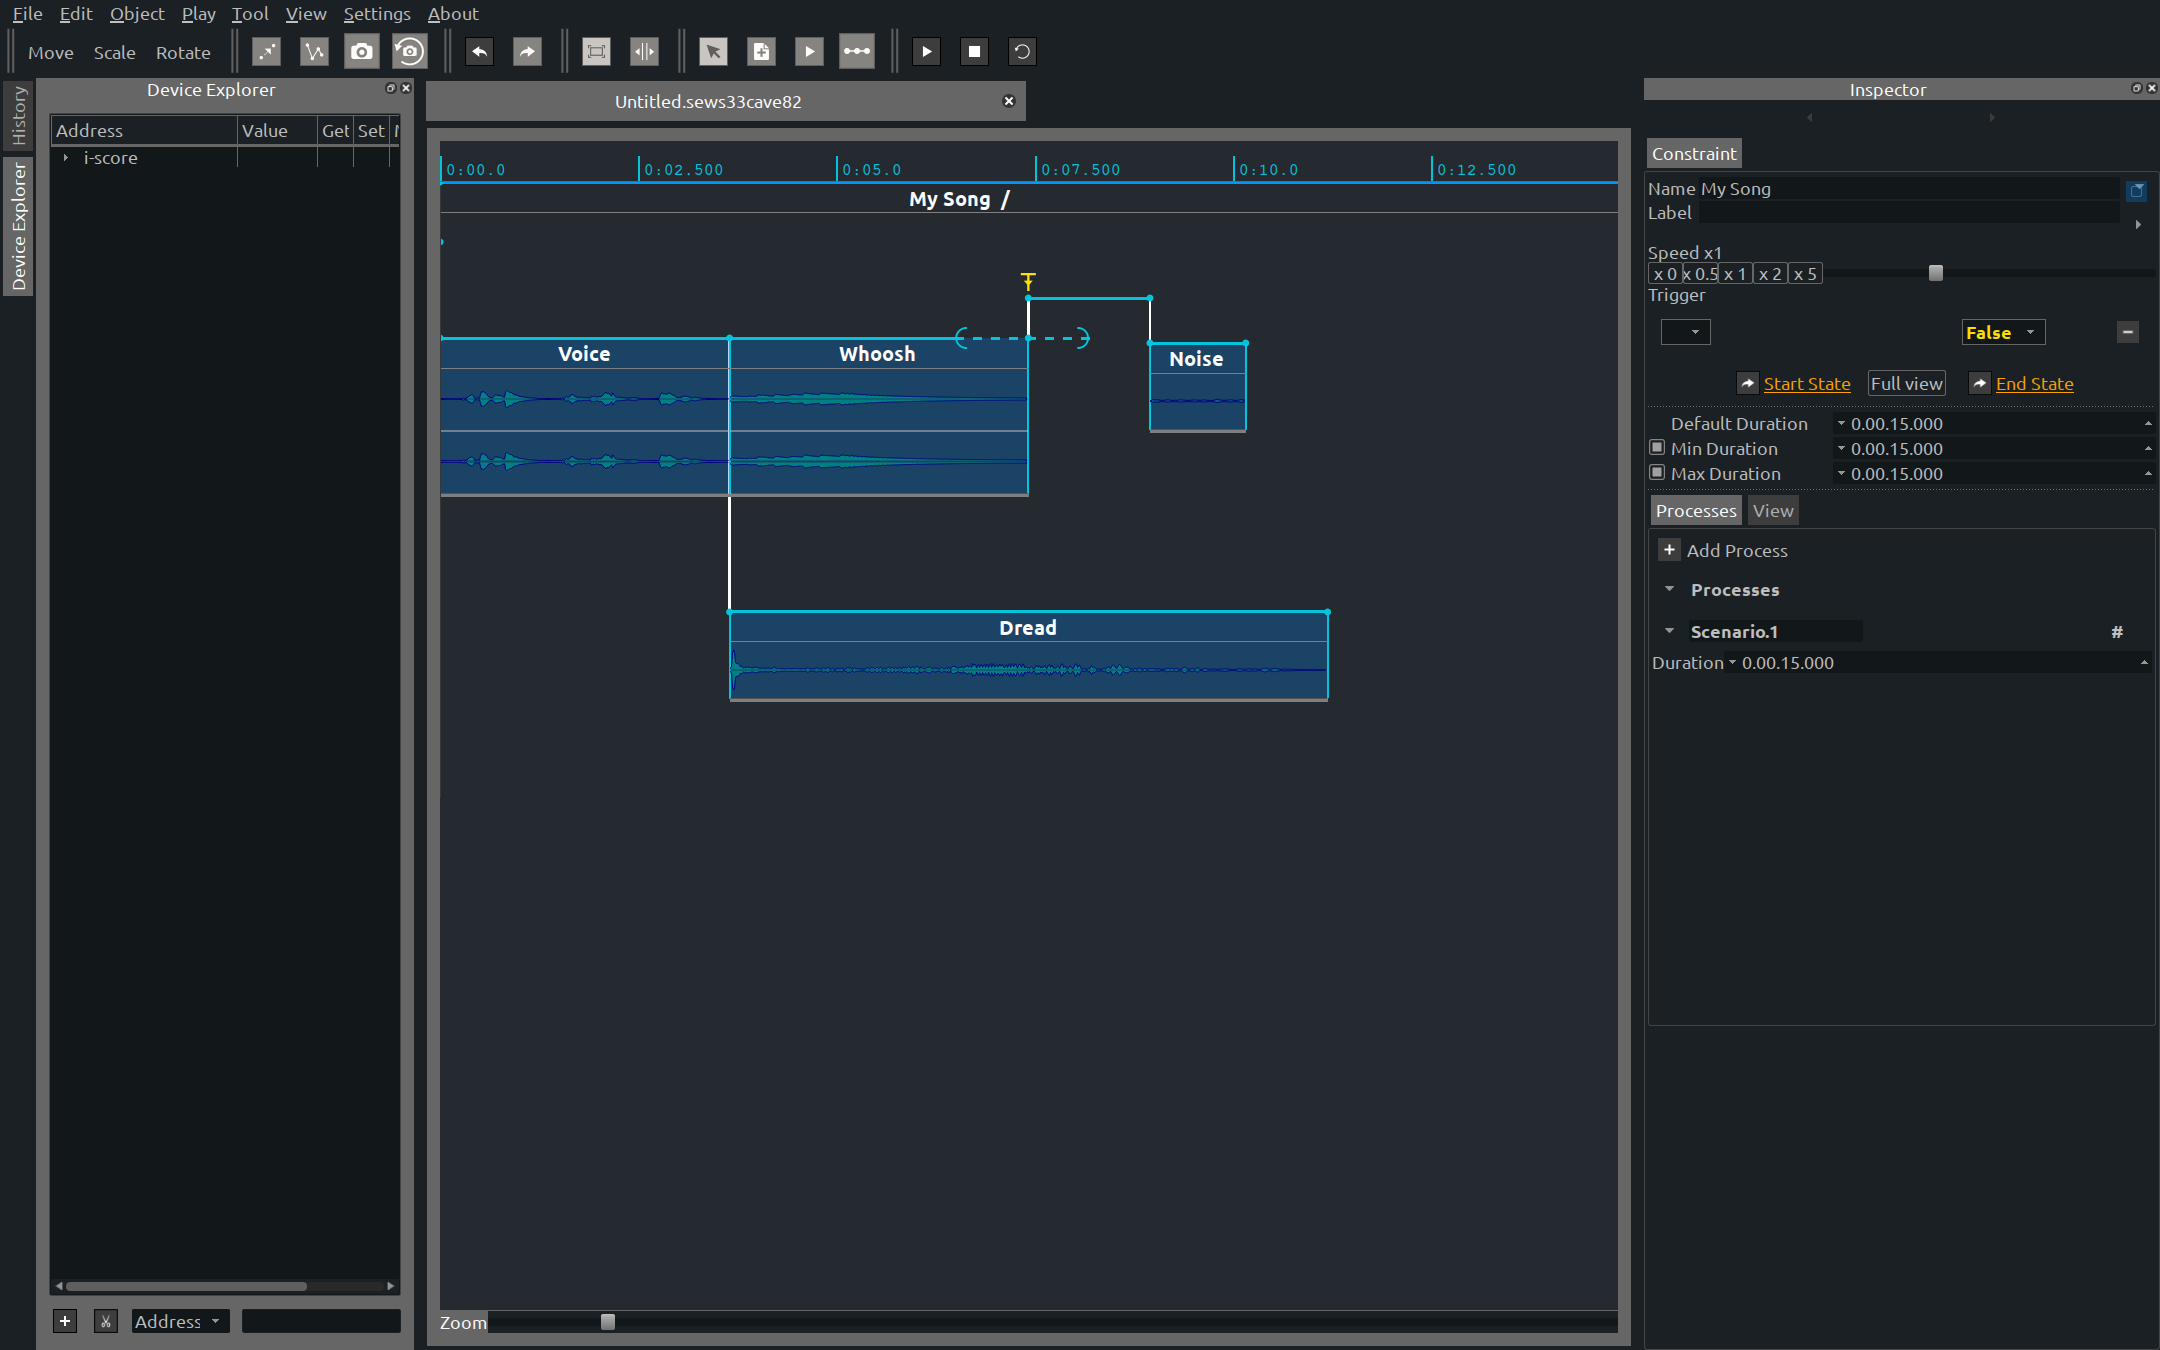
\includegraphics[width=\paperwidth]{images/screens/5.png}
    };
    \end{tikzpicture}
\end{frame}
\begin{frame}[plain]
    \begin{tikzpicture}[remember picture,overlay]
    \node[at=(current page.center)] {
        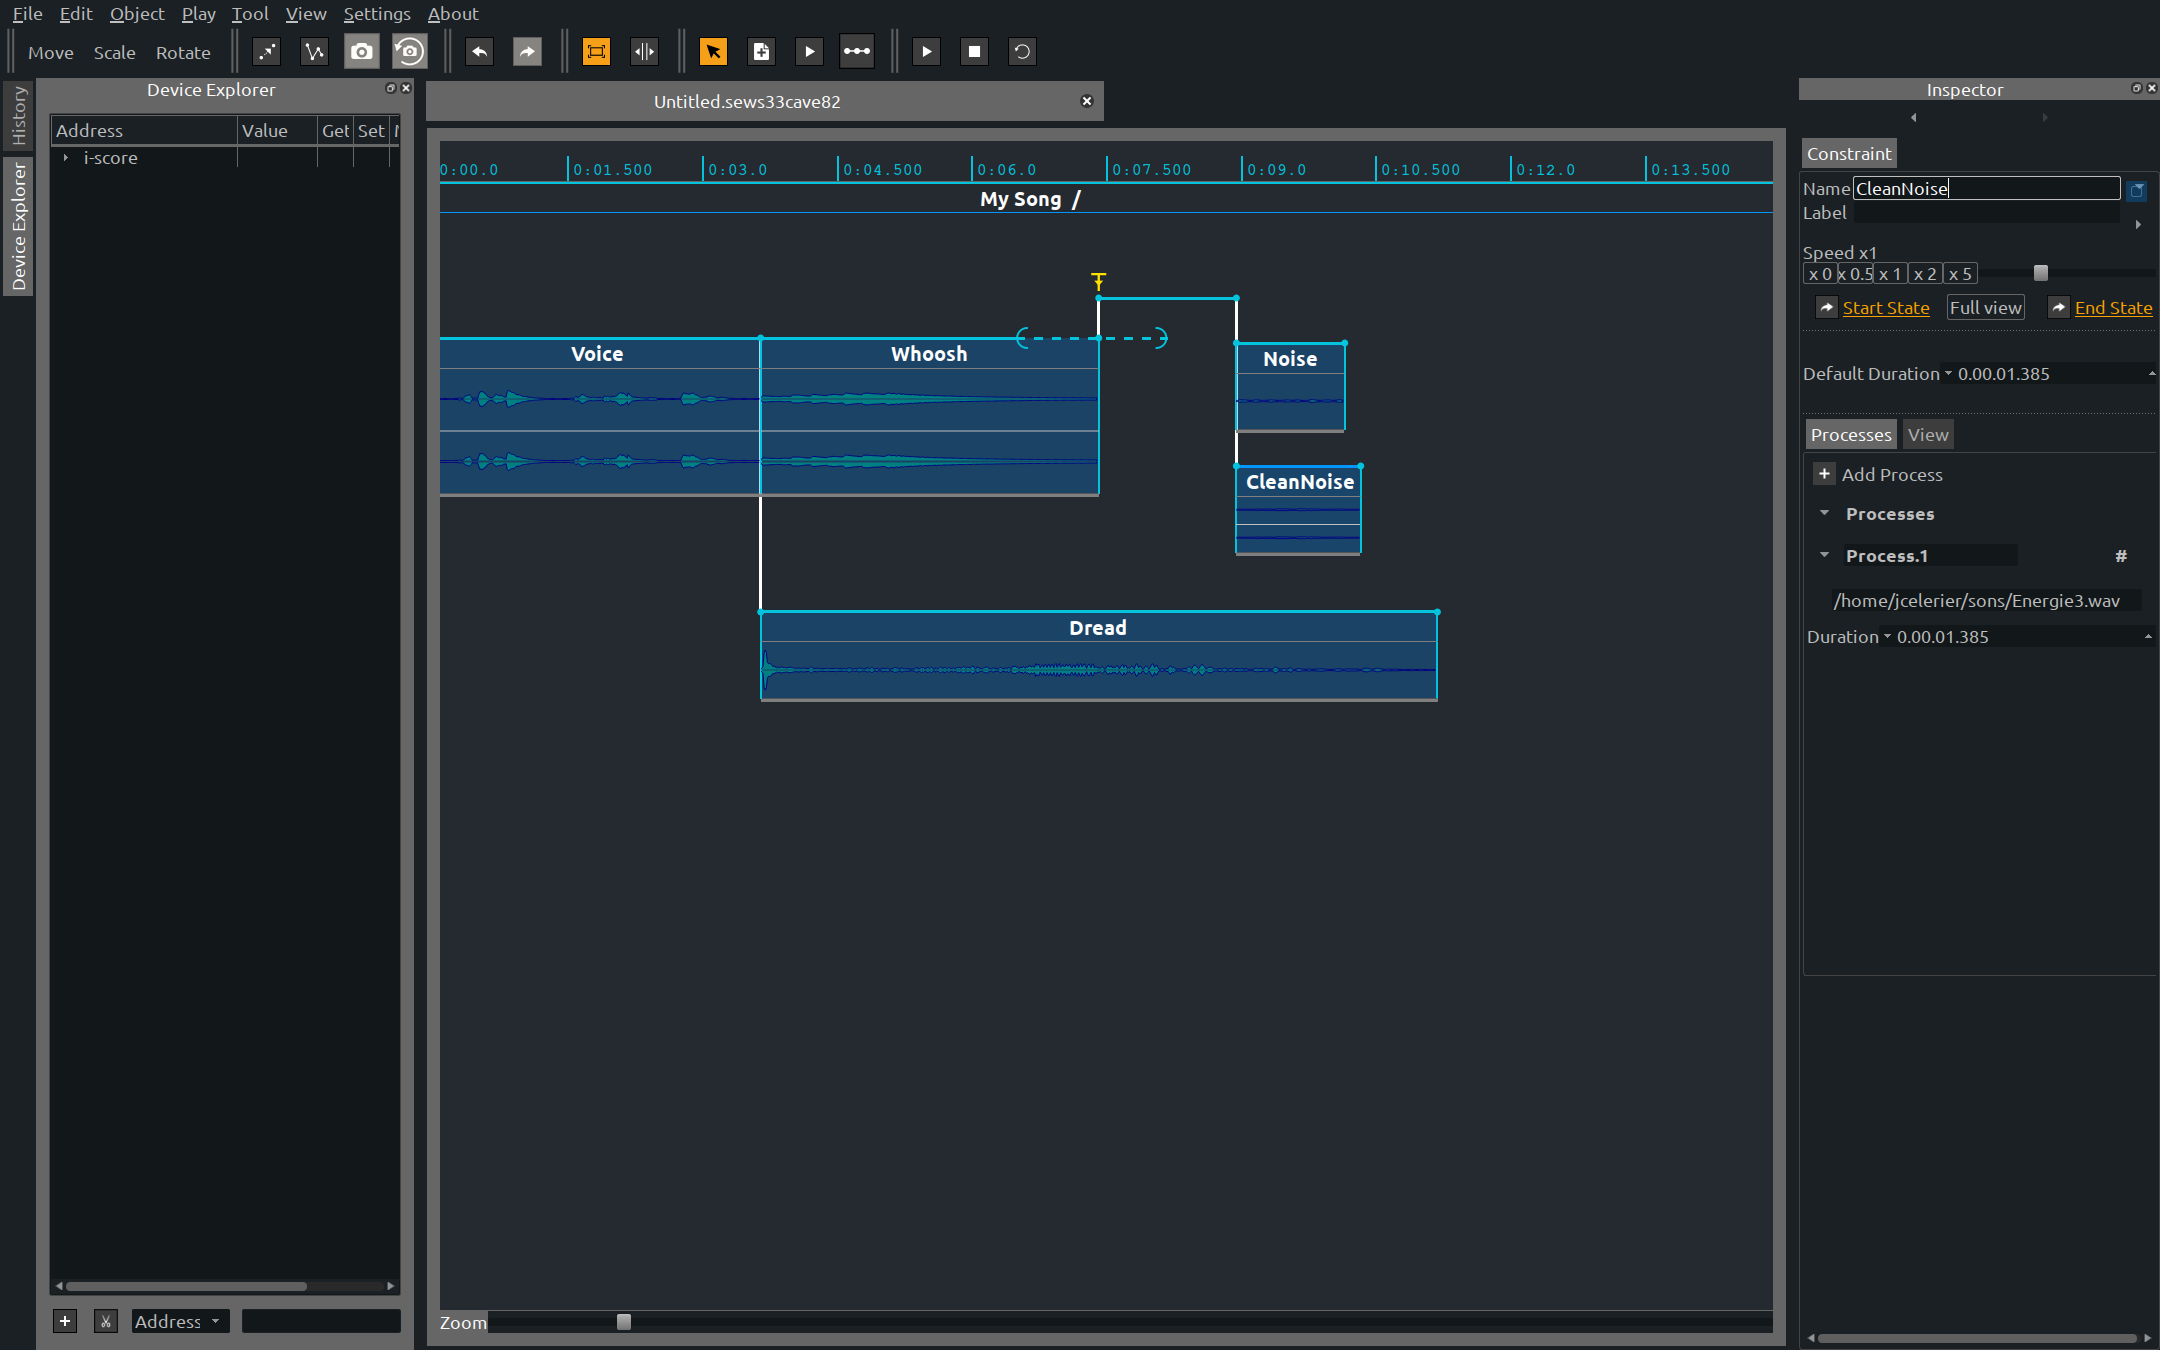
\includegraphics[width=\paperwidth]{images/screens/6.png}
    };
    \end{tikzpicture}
\end{frame}
\begin{frame}[plain]
    \begin{tikzpicture}[remember picture,overlay]
    \node[at=(current page.center)] {
        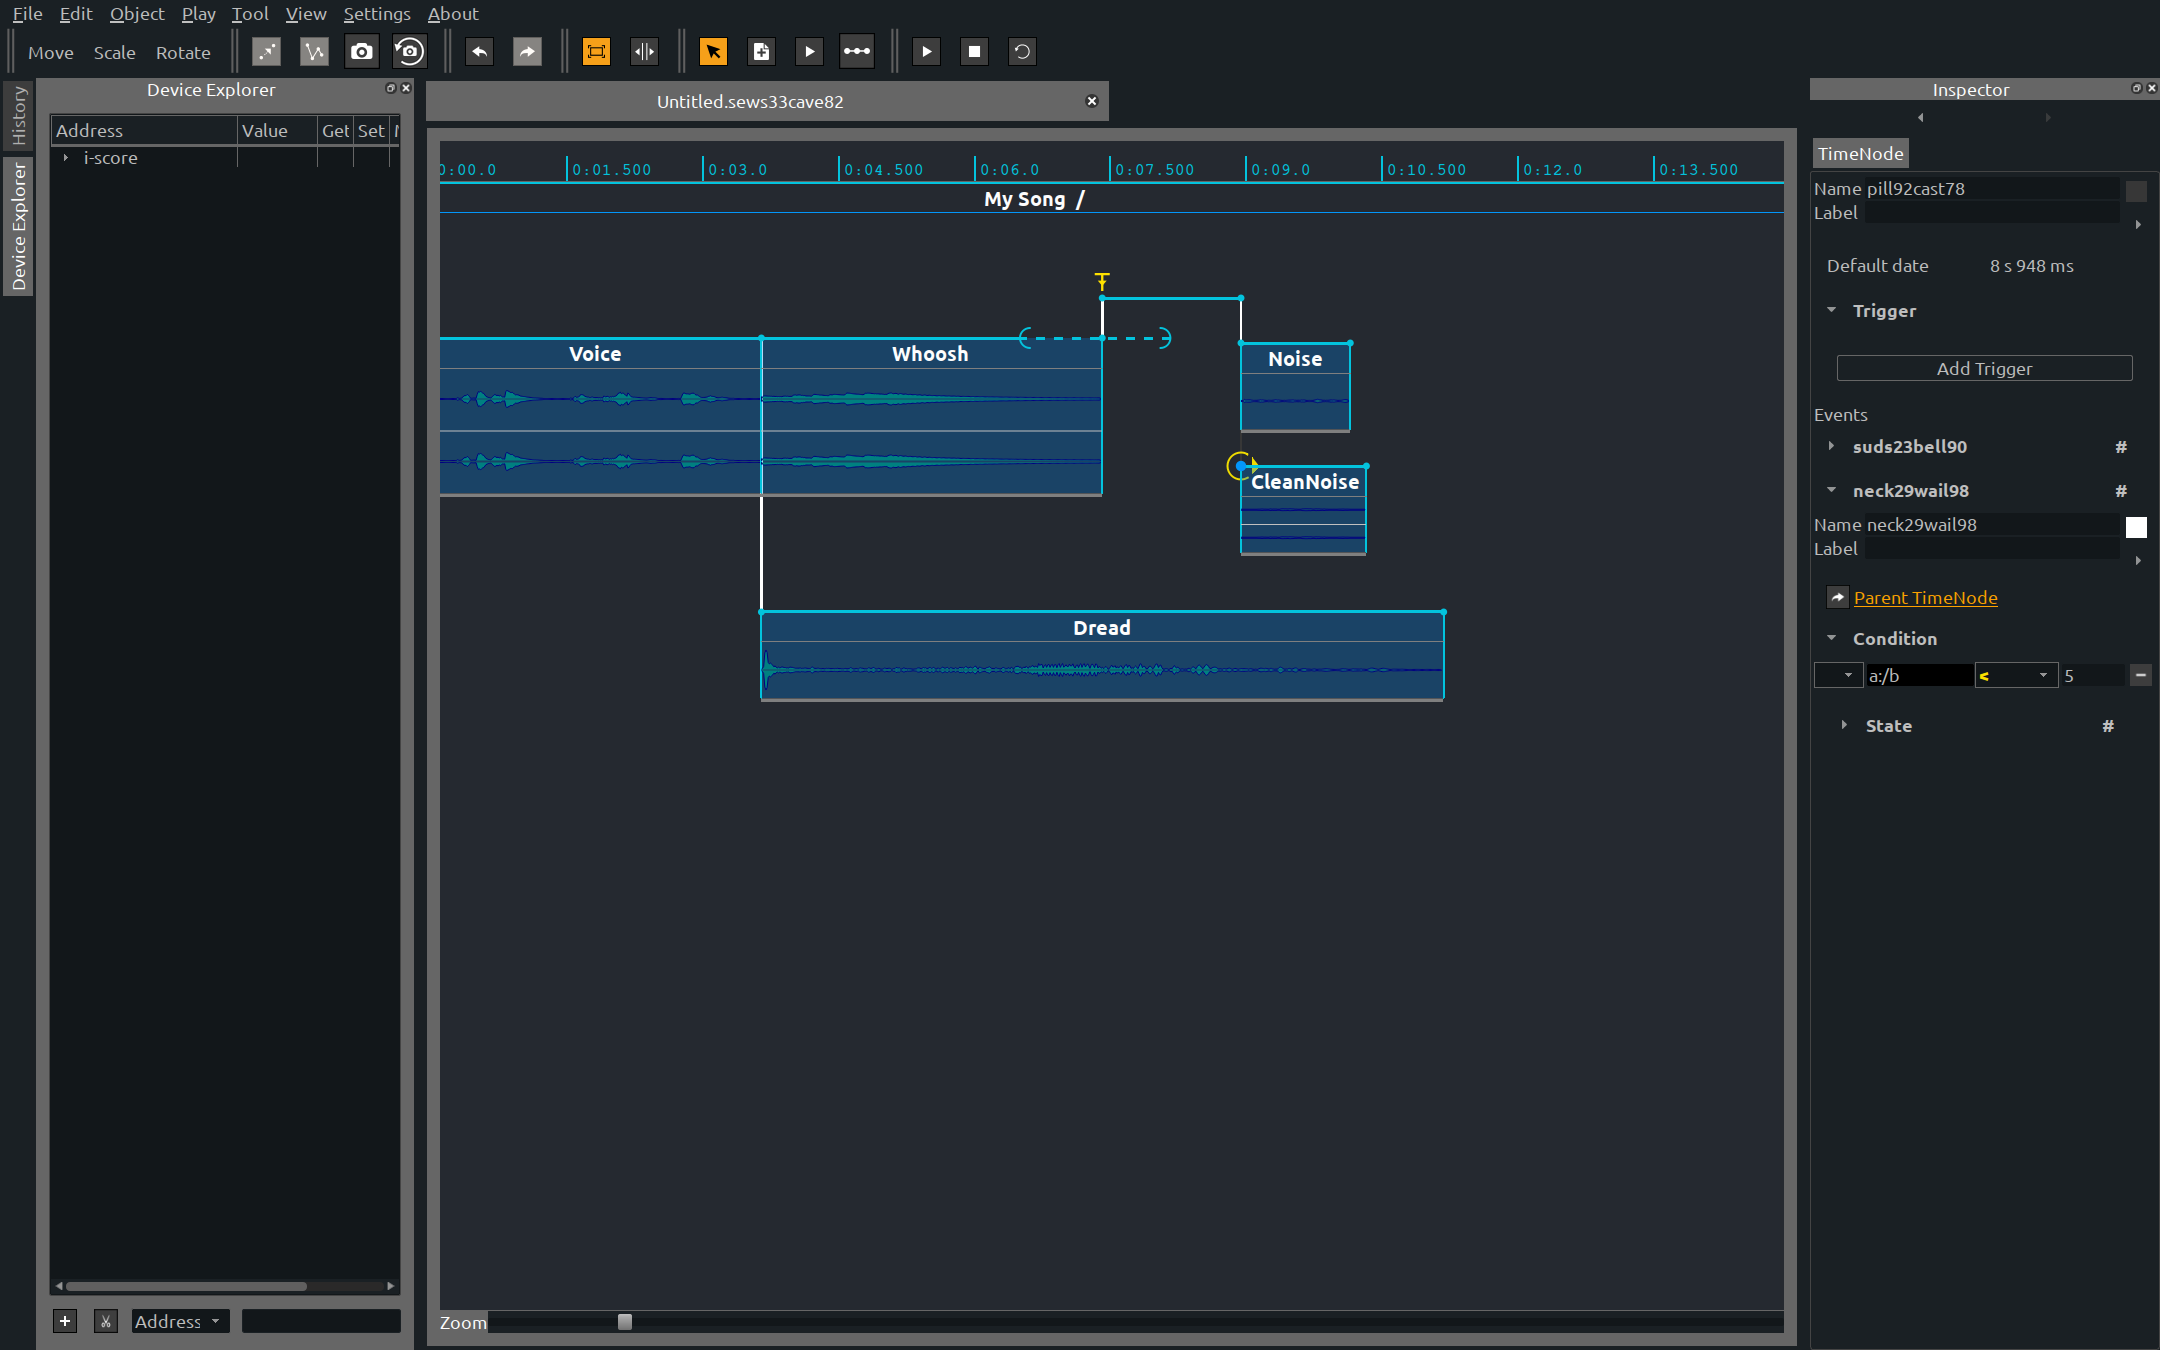
\includegraphics[width=\paperwidth]{images/screens/7.png}
    };
    \end{tikzpicture}
\end{frame}
\begin{frame}[plain]
    \begin{tikzpicture}[remember picture,overlay]
    \node[at=(current page.center)] {
        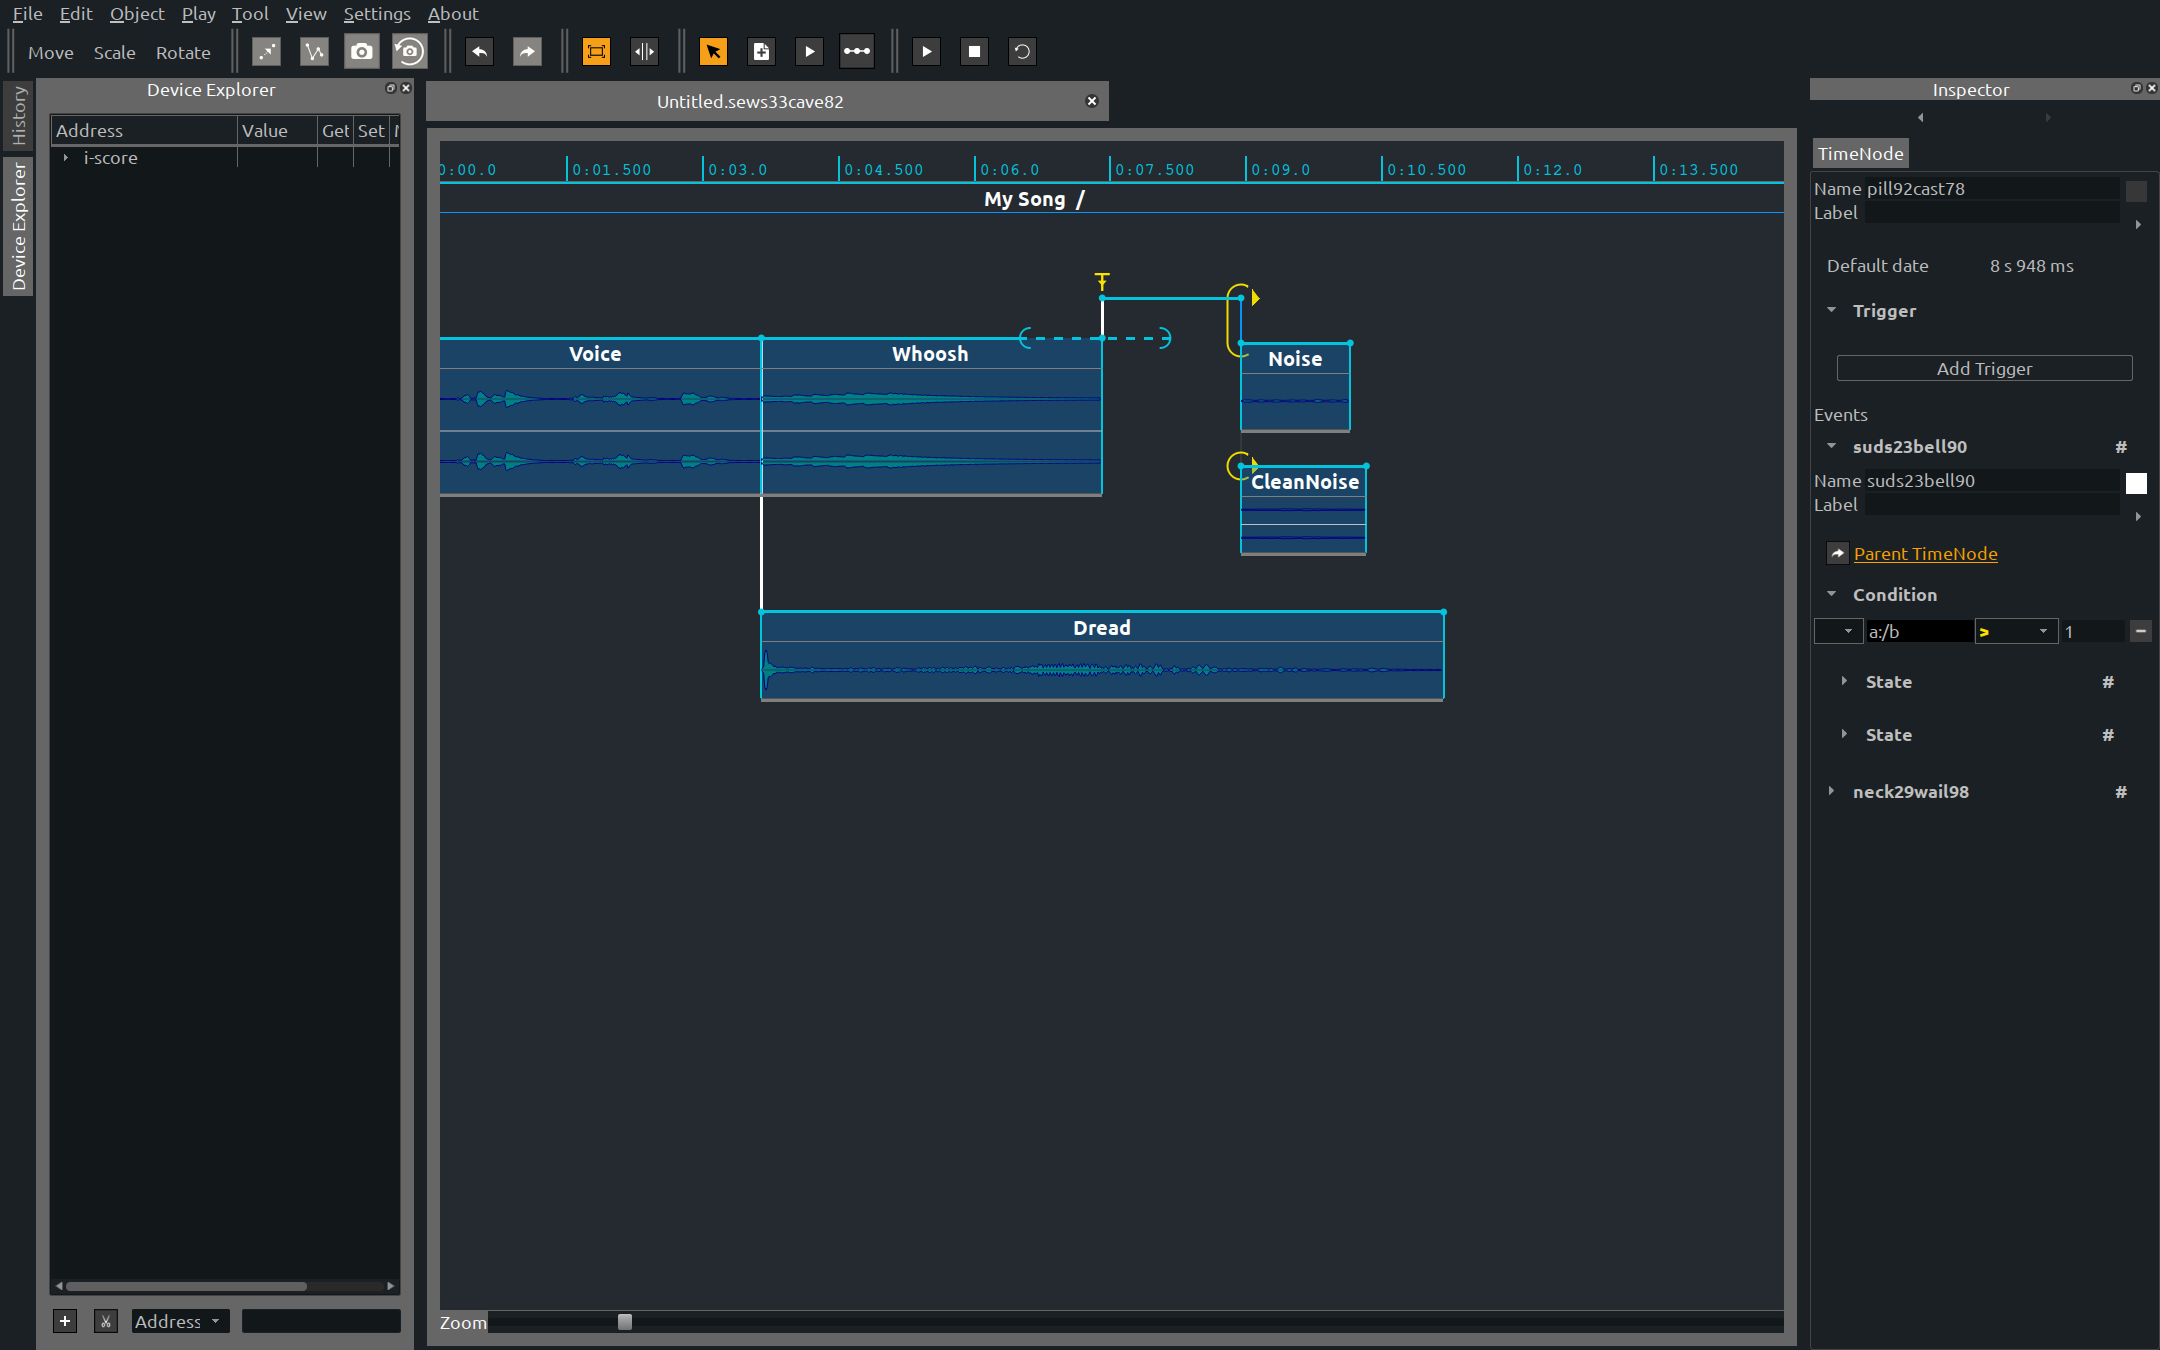
\includegraphics[width=\paperwidth]{images/screens/8.png}
    };
    \end{tikzpicture}
\end{frame}
\begin{frame}[plain]
    \begin{tikzpicture}[remember picture,overlay]
    \node[at=(current page.center)] {
        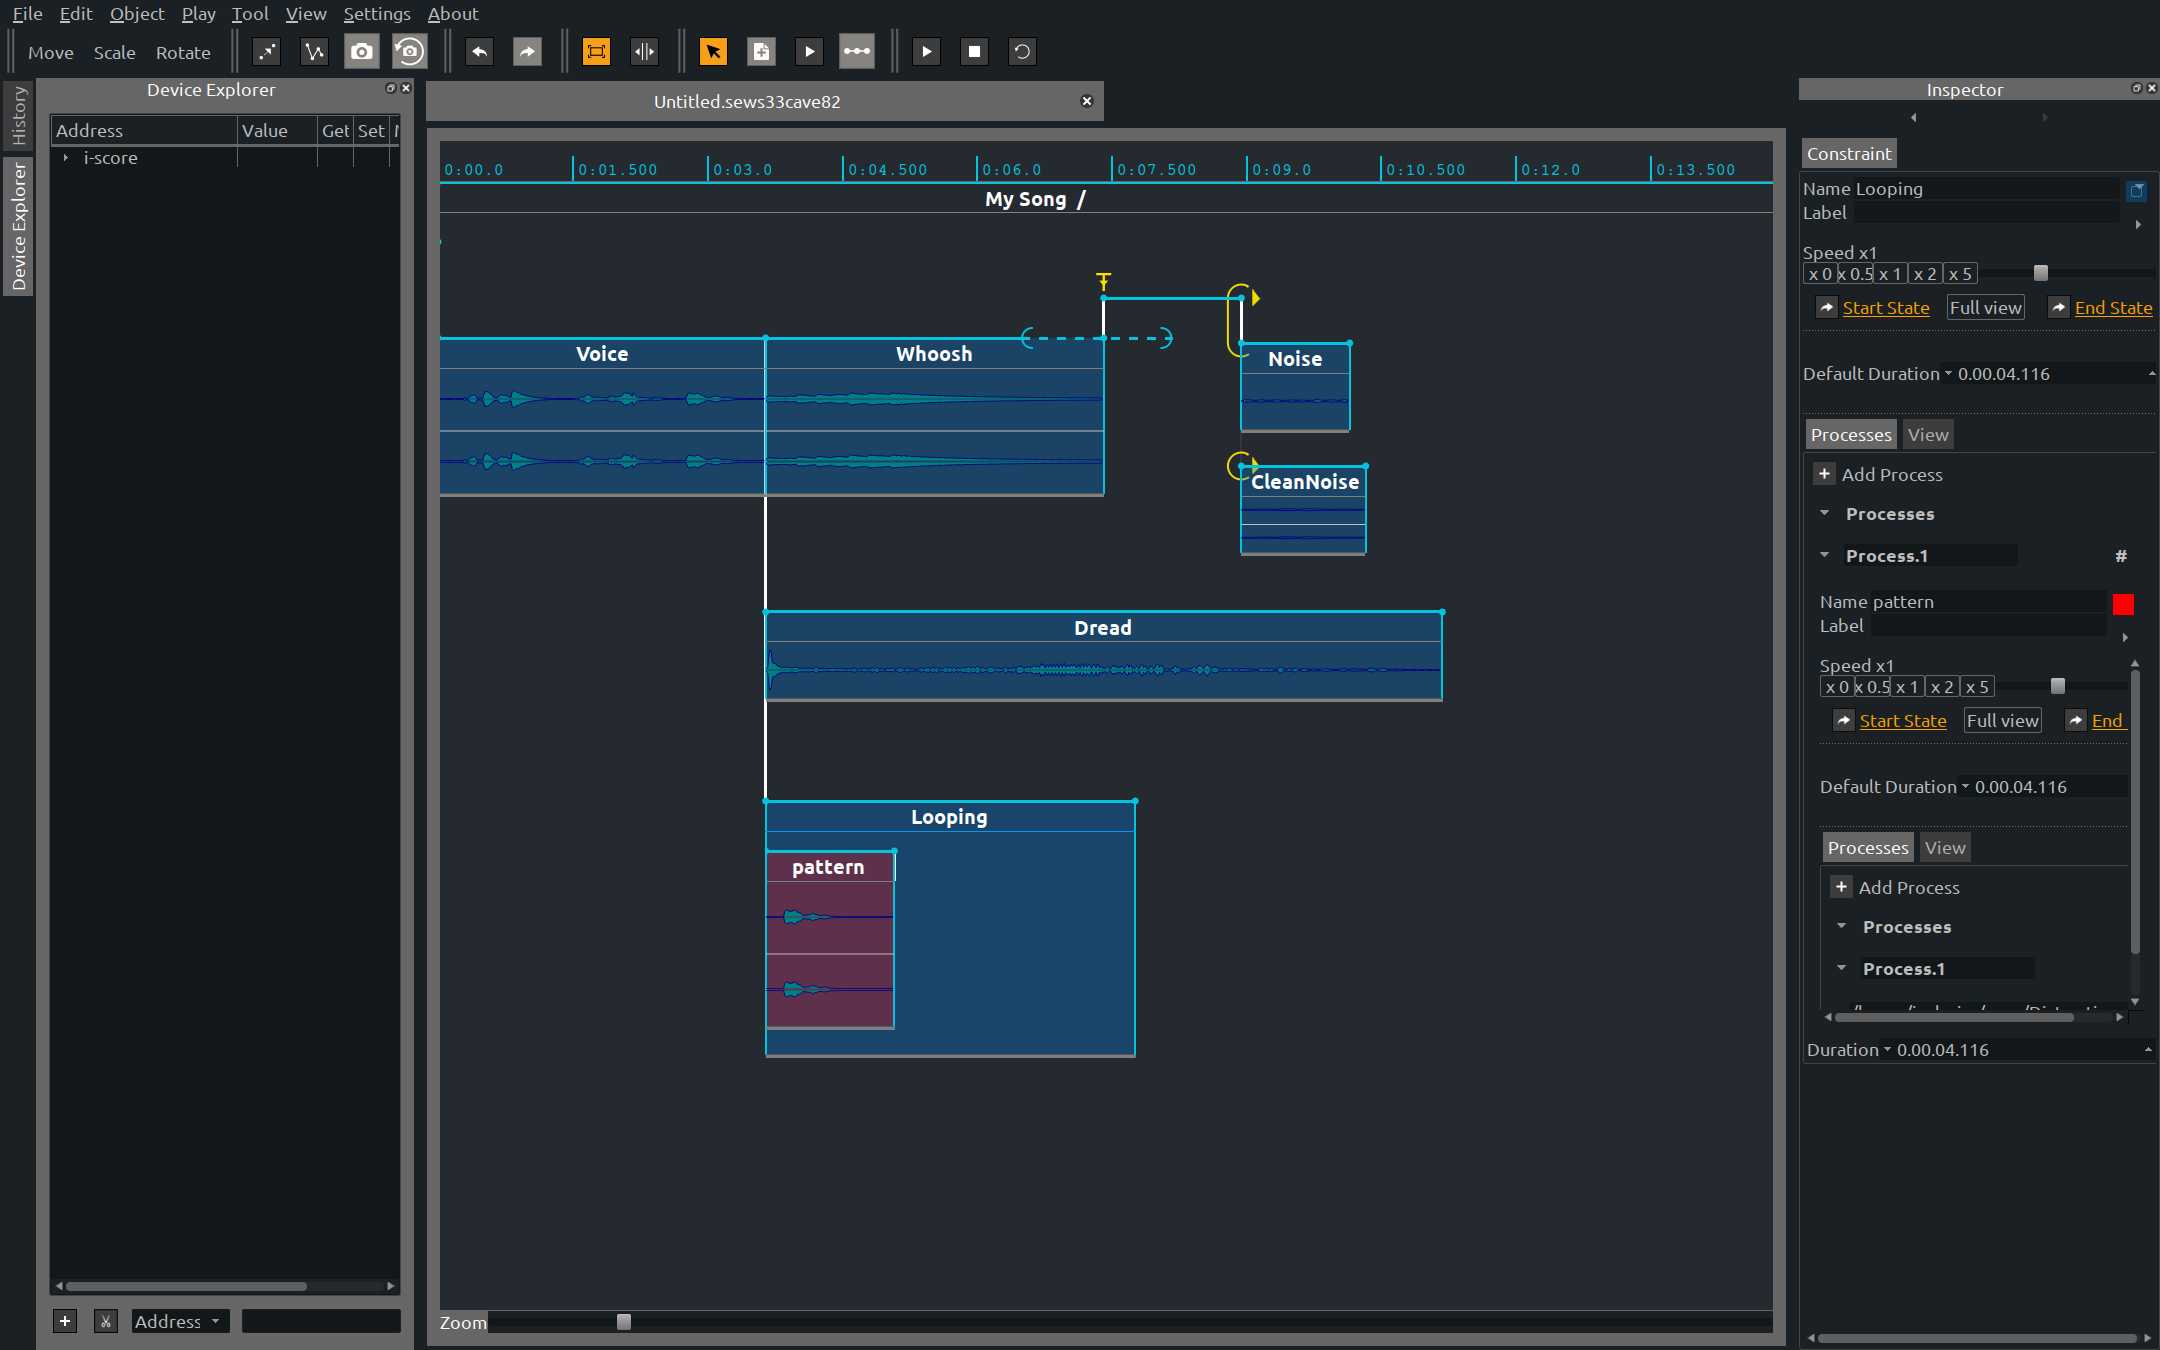
\includegraphics[width=\paperwidth]{images/screens/9.png}
    };
    \end{tikzpicture}
\end{frame}
\begin{frame}[plain]
    \begin{tikzpicture}[remember picture,overlay]
    \node[at=(current page.center)] {
        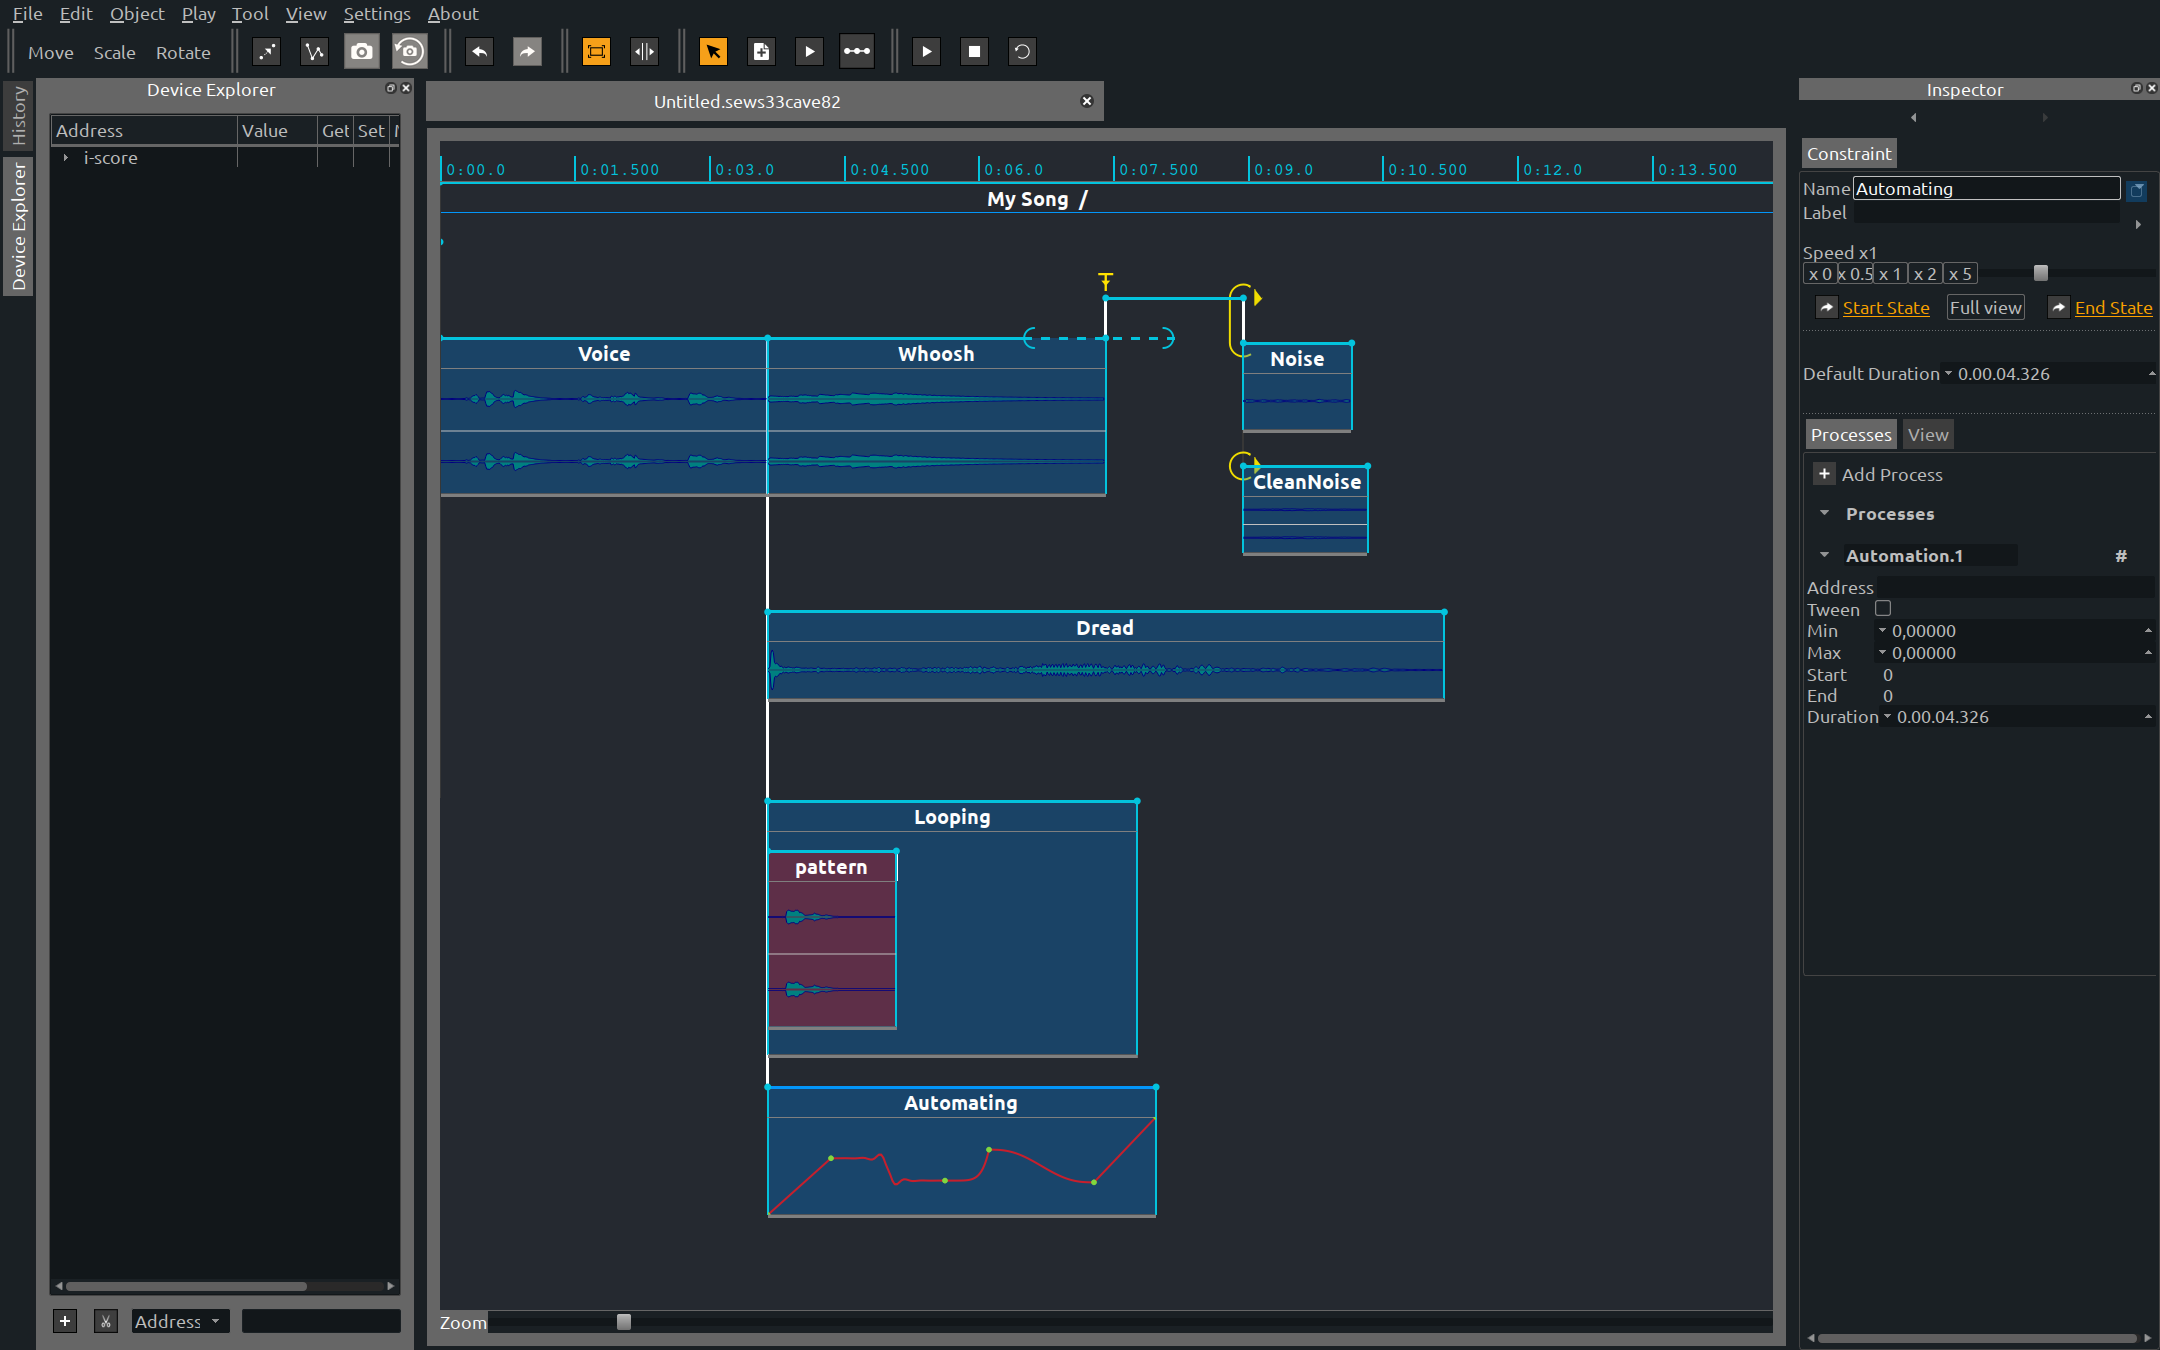
\includegraphics[width=\paperwidth]{images/screens/10.png}
    };
    \end{tikzpicture}
\end{frame}
\begin{frame}[plain]
    \begin{tikzpicture}[remember picture,overlay]
    \node[at=(current page.center)] {
        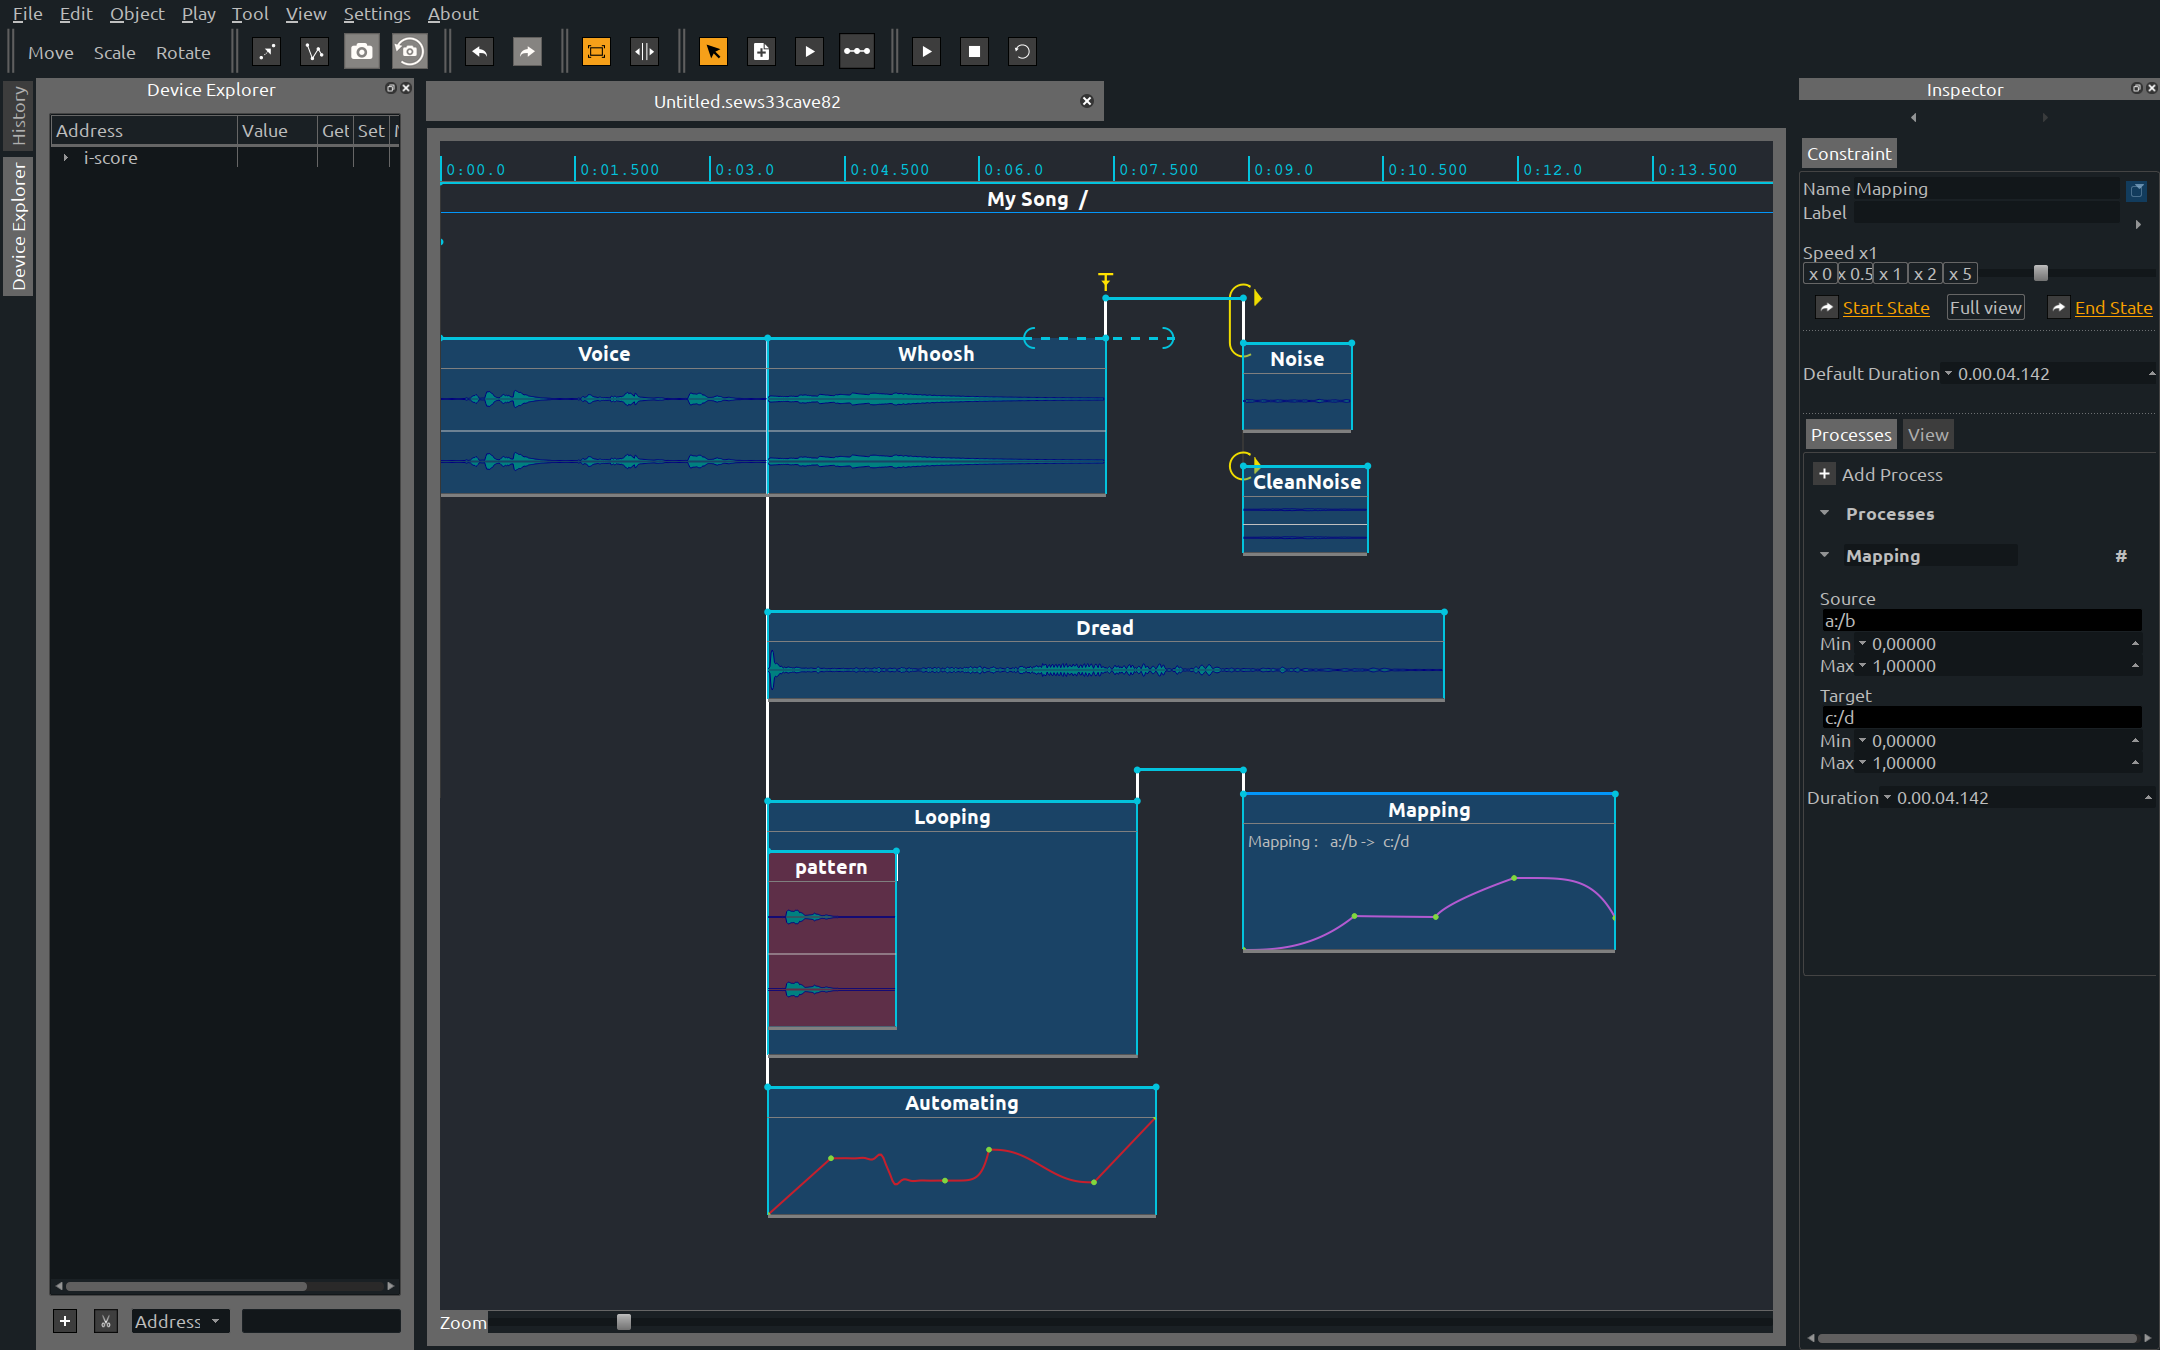
\includegraphics[width=\paperwidth]{images/screens/11.png}
    };
    \end{tikzpicture}
\end{frame}
\begin{frame}[plain]
    \begin{tikzpicture}[remember picture,overlay]
    \node[at=(current page.center)] {
        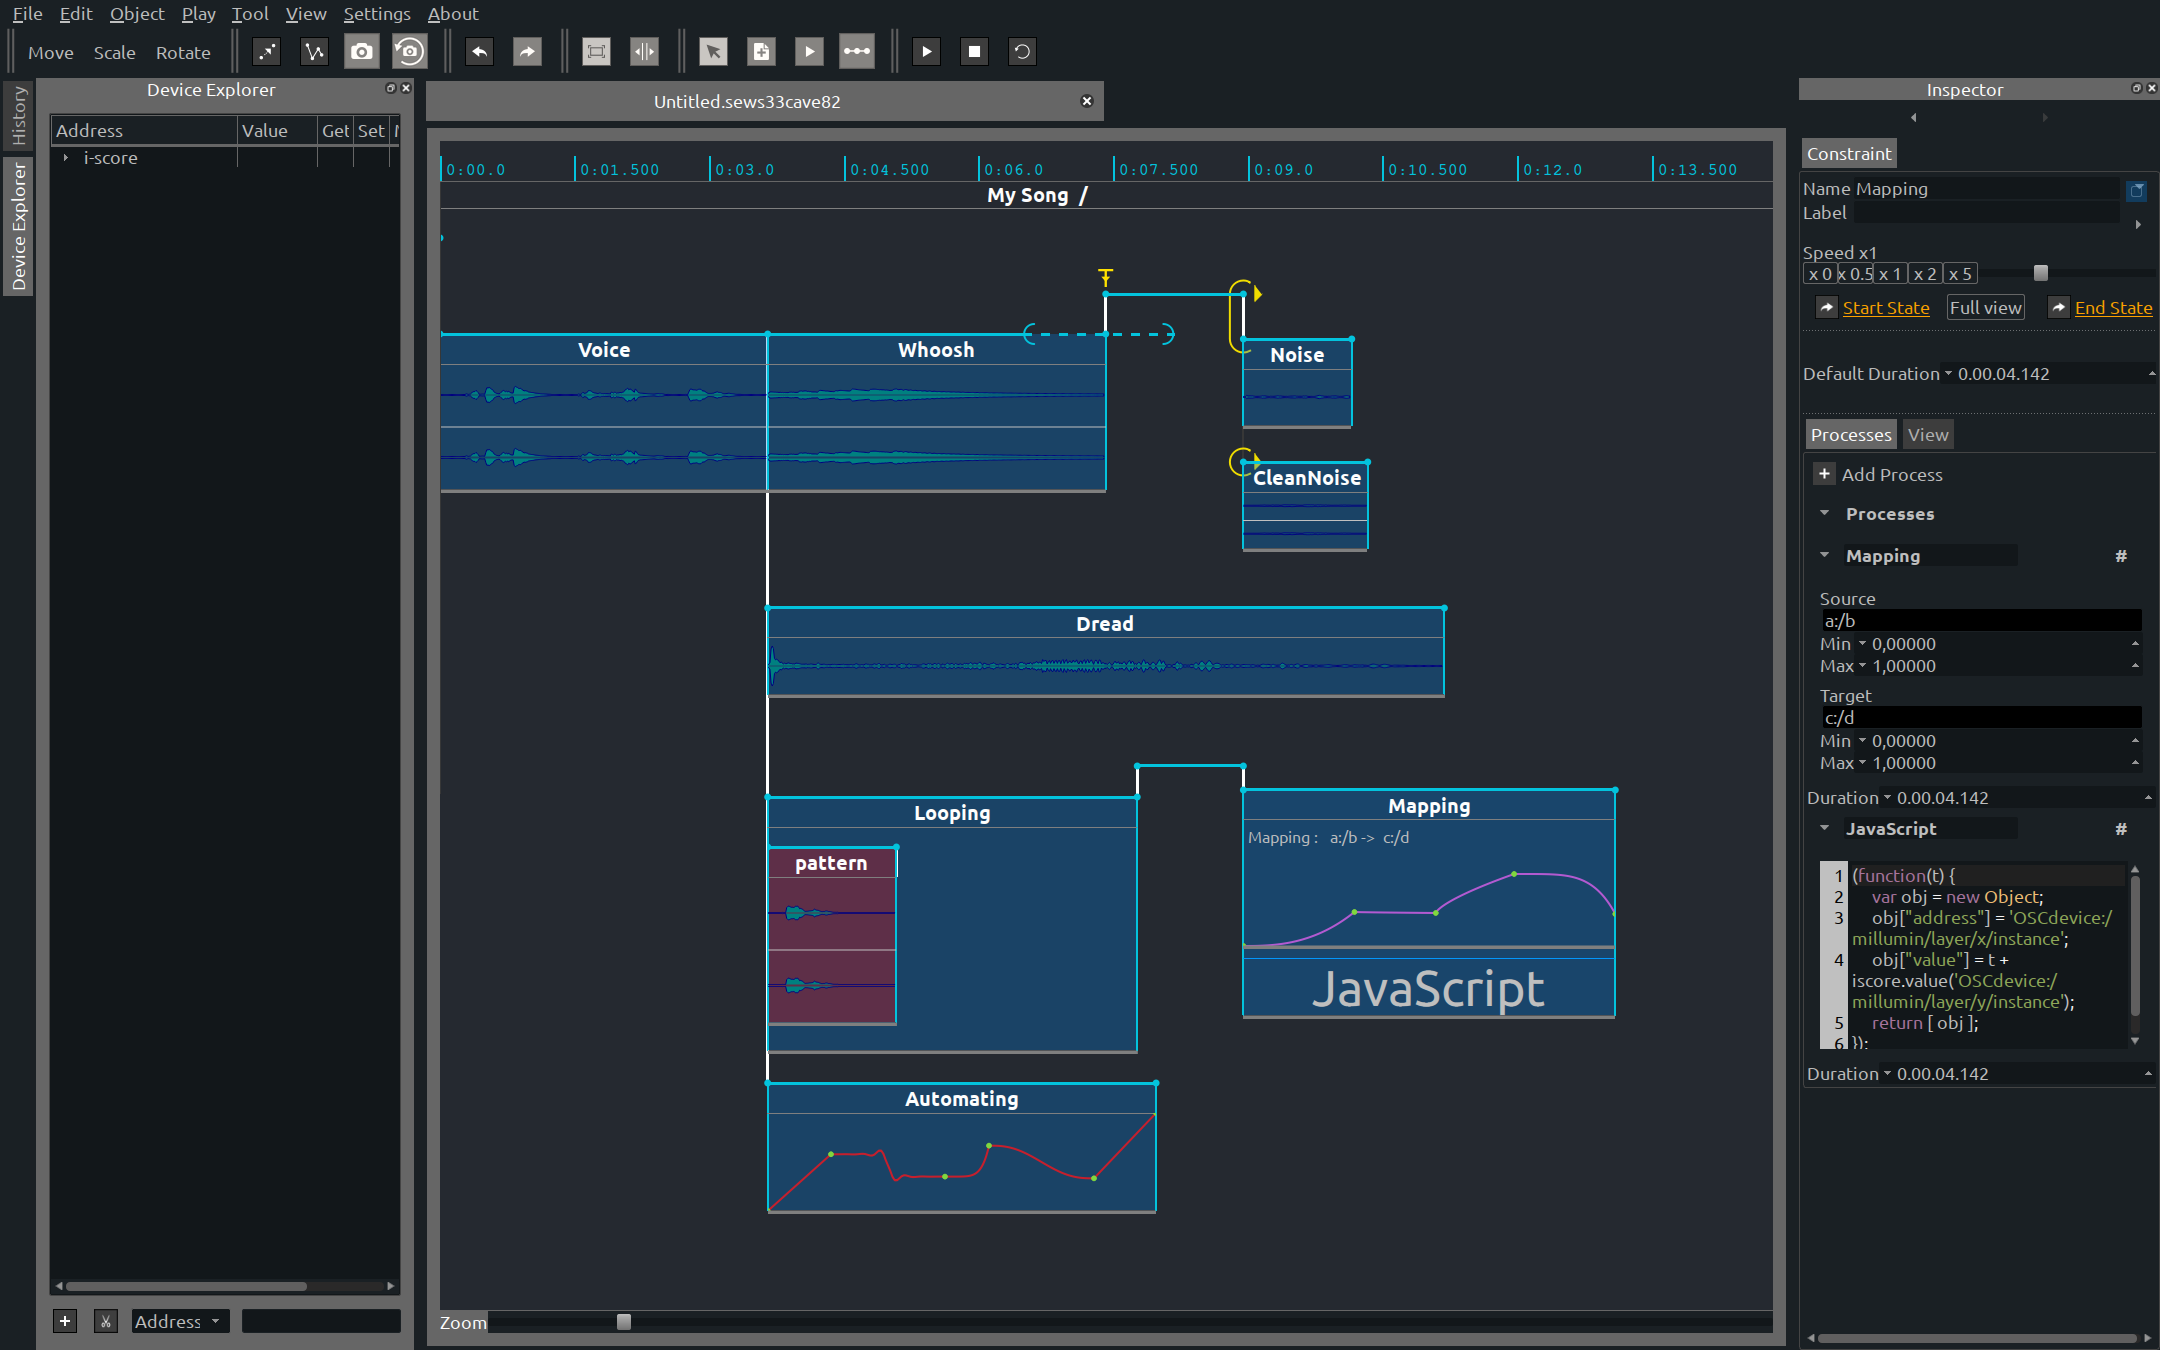
\includegraphics[width=\paperwidth]{images/screens/12.png}
    };
    \end{tikzpicture}
\end{frame}
\begin{frame}[plain]
    \begin{tikzpicture}[remember picture,overlay]
    \node[at=(current page.center)] {
        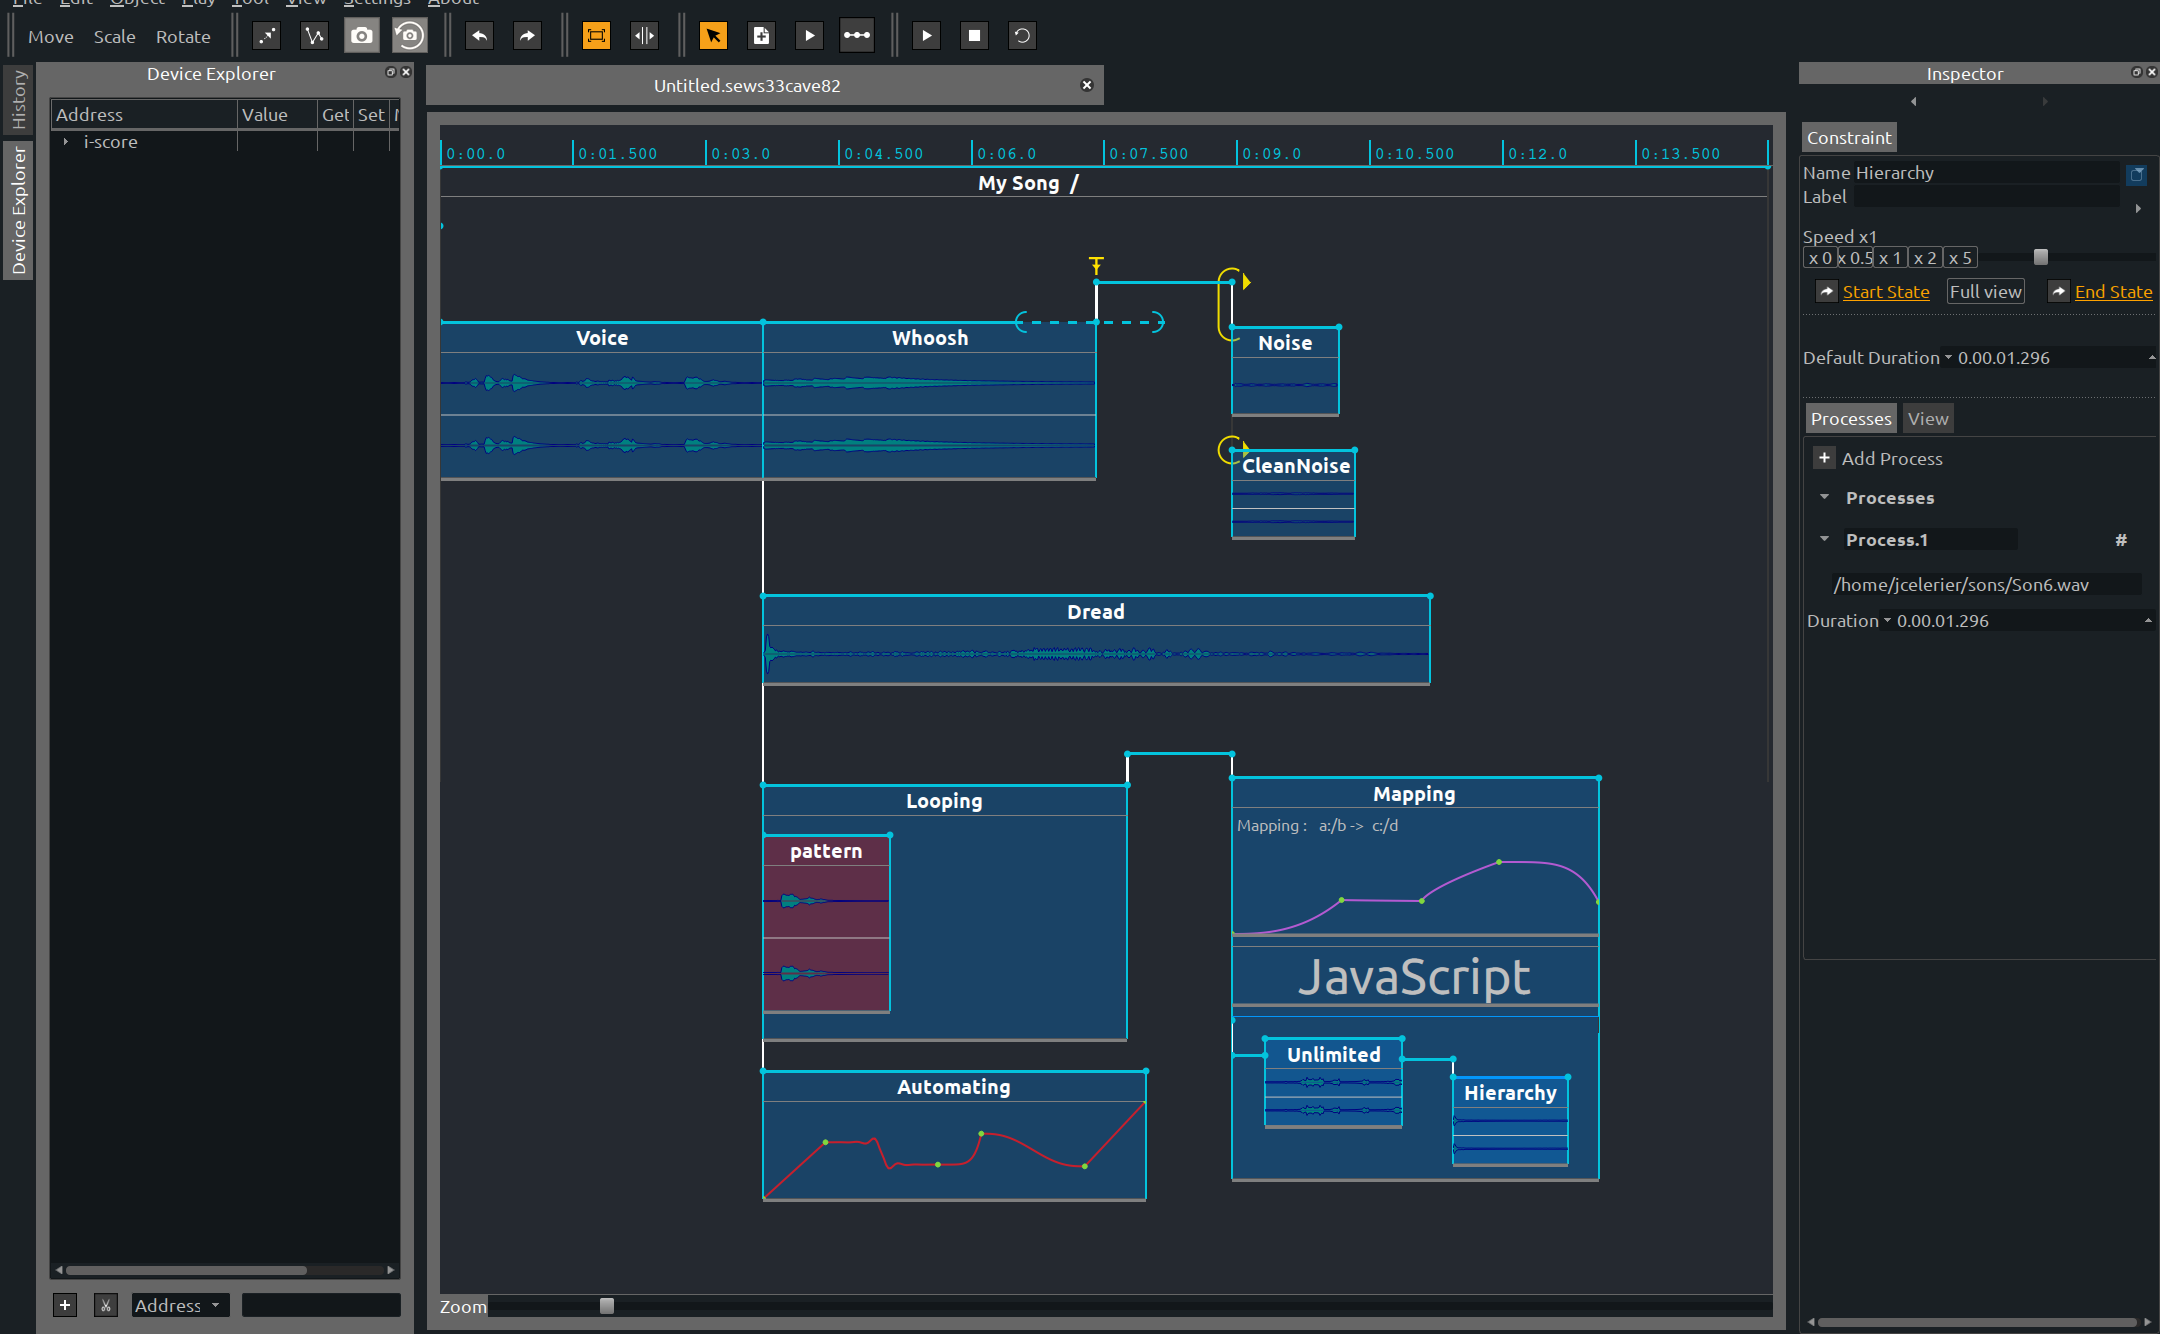
\includegraphics[width=\paperwidth]{images/screens/13.png}
    };
    \end{tikzpicture}
\end{frame}
\begin{frame}[plain]
    \begin{tikzpicture}[remember picture,overlay]
    \node[at=(current page.center)] {
        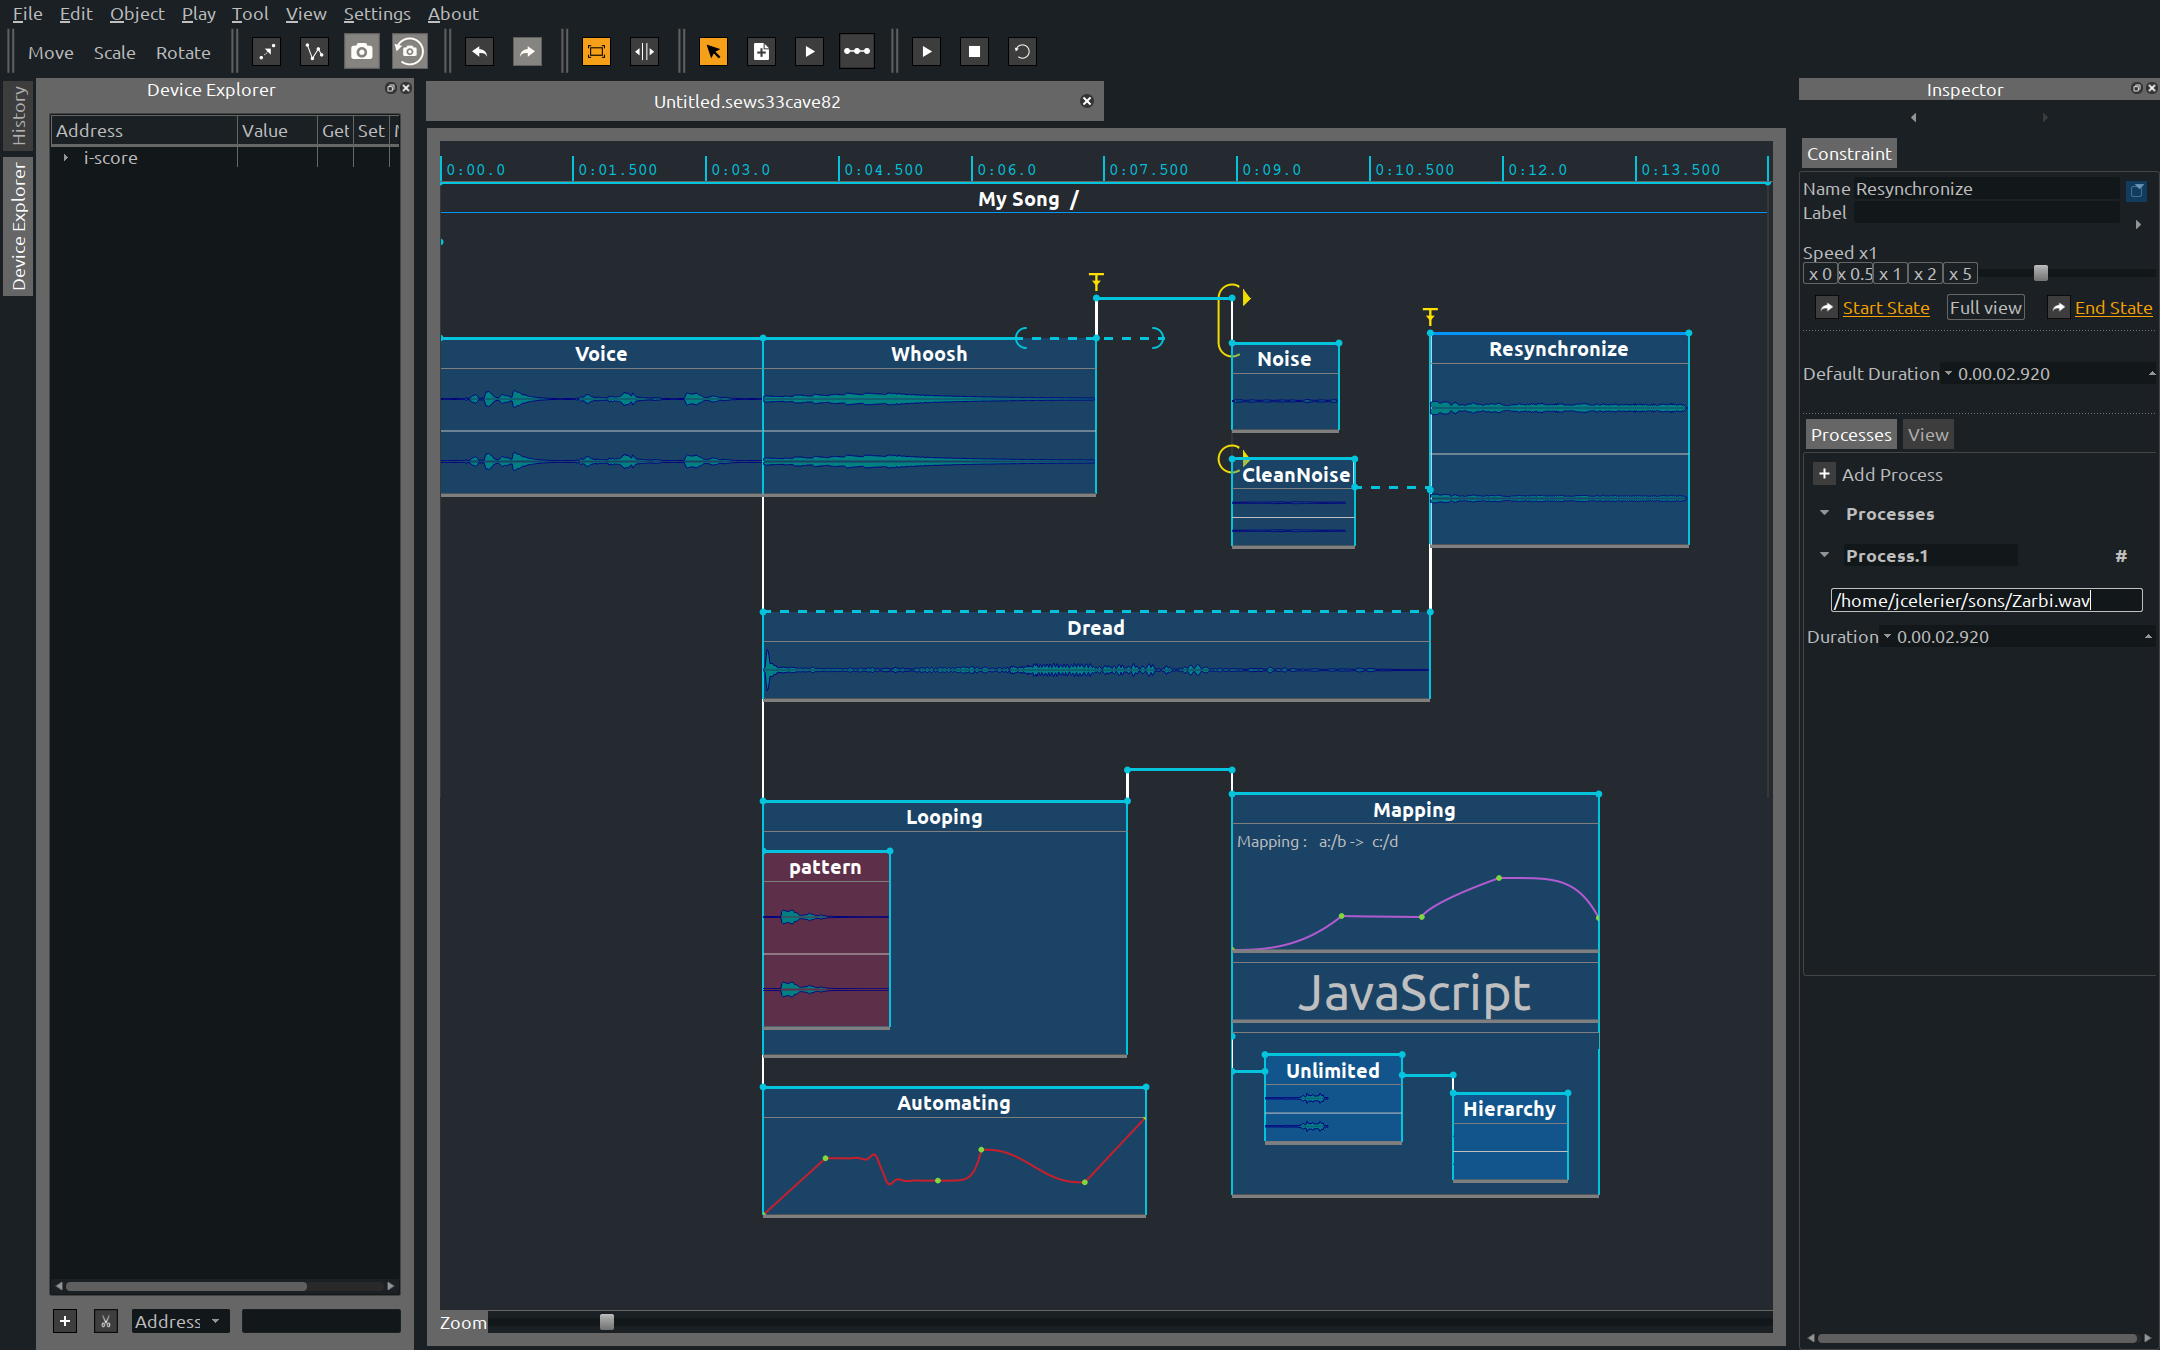
\includegraphics[width=\paperwidth]{images/screens/14.png}
    };
    \end{tikzpicture}
\end{frame}

\section{Description}

\begin{frame}	
    \frametitle{Origin}    
    \Large
    \begin{itemize}
        \item \textbf{i-score}~\\ \url{i-score.org}~\\$\rightarrow$ software for interactive show control.~\\~\\
        \item \textbf{LibAudioStream}\\ \url{github.com/sletz/libaudiostream}~\\$\rightarrow$ sequencer-as-a-library.~\\~\\
        \item \textbf{Audio plug-in} for i-score.
    \end{itemize}   
     
\end{frame}


\begin{frame}
    \Huge
    \centering{Vocabulary}
\end{frame}
    
    
\begin{frame}[plain]
    \begin{tikzpicture}[remember picture,overlay]
    \node[at=(current page.center)] {
        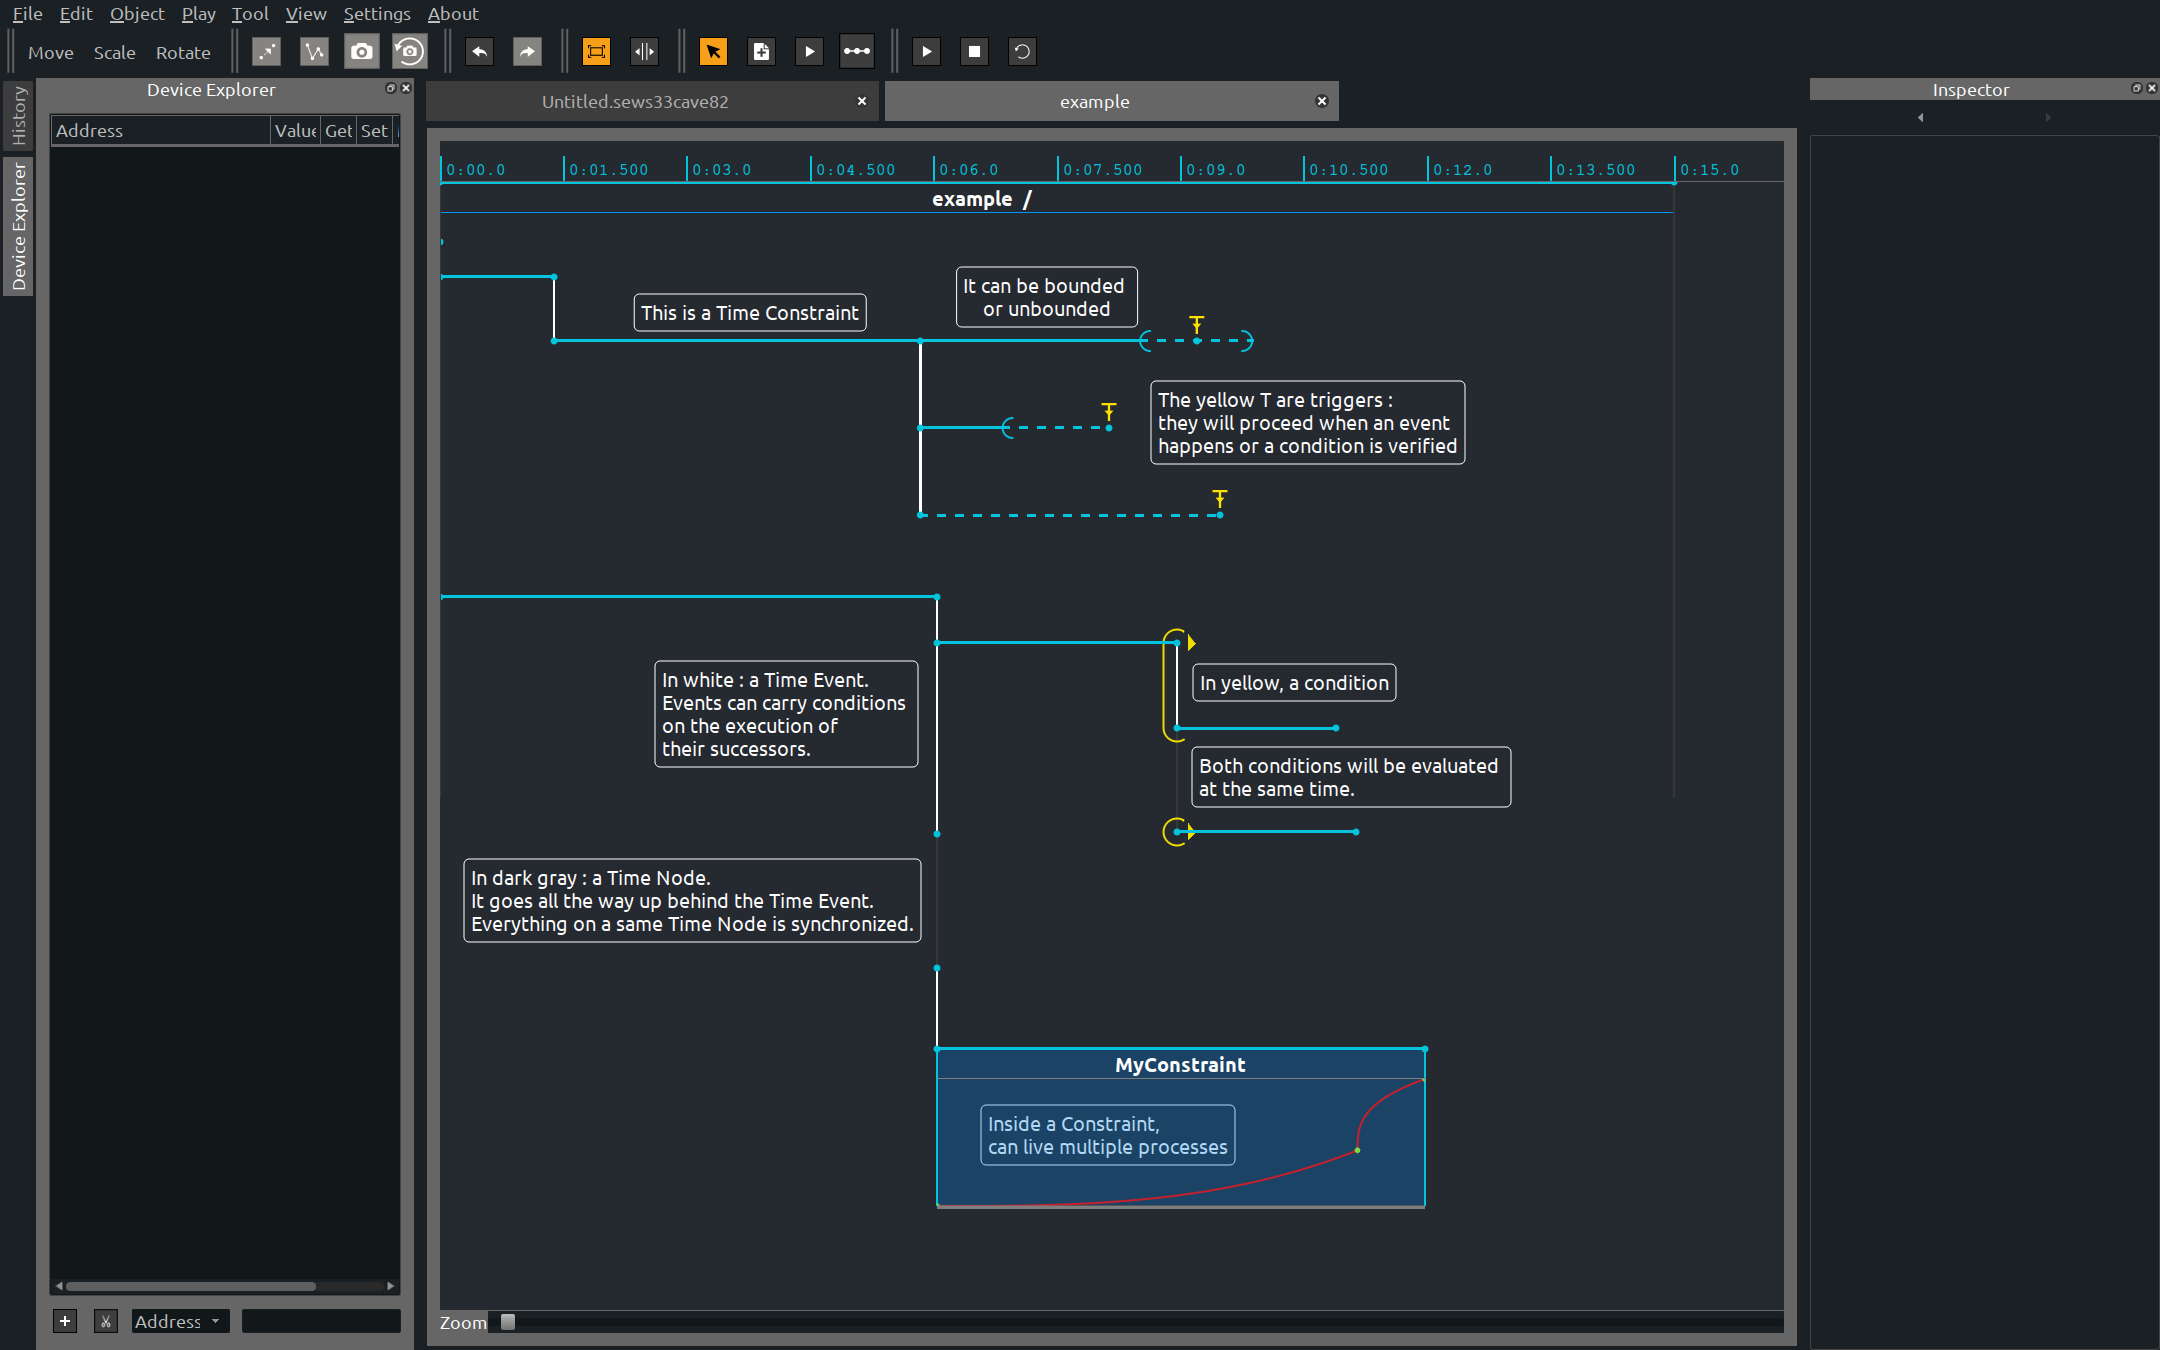
\includegraphics[width=1.5\paperwidth]{images/screens/example.png}
     };
     \end{tikzpicture}
\end{frame}

\subsection{Audio processes}
\begin{frame}	
    \frametitle{Audio processes}    
    \LARGE
    \begin{itemize}
        \item Soundfile reading.
        \item Real-time input.
        \item Effect chains (Faust, LV2 in-progress).
        \item Audiograph features~\\$\rightarrow$ send and return from different points in the score.
        \item Mixing.
    \end{itemize}    
\end{frame}

\section{Method}
\begin{frame}
    \frametitle{The i-score audio graph}    
    \Large
    \begin{itemize}
        \item Audiostreams should be available for reading everywhere in the score : \\ $\rightarrow$ \textbf{flowgraph}.
        \item Not shown: it is not the main use case but a tool. UI focus is on the \textbf{temporal} aspect.
        \item For now the graph creation is \textbf{static}.
    \end{itemize}    
\end{frame}

\begin{frame}
    \frametitle{The i-score audio graph : mixing}    
	\Large
	
    Mixing unit : the temporal constraint.
    
    \begin{itemize}
        \item Constraints mixes themselves in their parent process.
        \item Processes mixes themselves in their parent constraint.
    \end{itemize}
    
	\begin{figure}
		\centering
		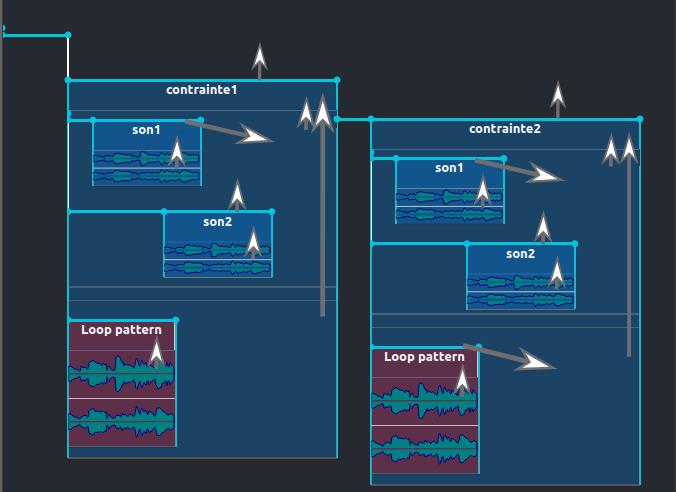
\includegraphics[width=0.5\textwidth]{images/mixage.png}
		\caption{Objects mix themselves together following the arrows}
	\end{figure}
\end{frame}


\section{Demo}
\begin{frame}
    \Huge
    \centering{Demo}
\end{frame}

\begin{frame}
	\frametitle{Future} 
	\Large
	\begin{itemize}
		\item<1> Integrated input recording.
		\item<2> Real-time audio input delaying and reuse.
		\item<3> Deep MIDI integration, piano roll, etc.
		\item<4> Hierarchic temporal signatures.
		
	\end{itemize}
\end{frame}    


\begin{frame}[allowframebreaks]%in case more than 1 slide needed
    
    %remove the icon
    \setbeamertemplate{bibliography item}{}
    
    %remove line breaks
    \setbeamertemplate{bibliography entry title}{}
    \setbeamertemplate{bibliography entry location}{}
    \setbeamertemplate{bibliography entry note}{}
    
    {\footnotesize
        \nocite{*}
        \bibliographystyle{IEEEtran}
        \bibliography{smc2016}
    }
\end{frame}

\begin{frame}
    \frametitle{Links} 
    \Large
    \begin{itemize}
        \setlength\itemsep{1em}
        \item \textbf{Audio extension ({\unicodefun Mac, Linux, soon Windows})} :~\\
        \url{github.com/OSSIA/iscore-addon-audio} 
        \item \textbf{i-score} :~\\
         \url{i-score.org}
    \end{itemize}
        
    \centering
    \vspace{2em}
    \Large{Thanks ! Questions ?}
    \vspace{2em}
    
    \tiny{Uses the Beamer 'simple' theme, Facundo Muñoz; and Mozilla's Fira font family}
\end{frame}
\end{document}
